%!TEX root=../../main.tex


\subsection{The frameworks during setup and benchmark}
We would like to raise some issues we encountered first while installing and configuring and second while running the different frameworks.

\begin{enumerate}
	\item During setup and benchmark of Gemini, we encountered several bugs in the cloned repository. These include non zero-terminated strings or even missing return statements.

	The errors rendered the code as-is unable to perform calculations, forcing us to fork the repository and modify the source code. A repository with our changes can be found \href{https://github.com/jasc7636/GeminiGraph}{here}\footnote{\url{https://github.com/jasc7636/GeminiGraph}}.

	\item Furthermore, we would like to address the setup of Hadoop for Giraph. It requires multiple edits in \texttt{xml} files that aren't easily automized. This makes the setup rather time consuming, especially if reconfiguration is needed later on.
	\item In order for Giraph to run, several Java tasks (the Hadoop infrastructure) have to be constantly running in the background. While we don't expect this to have a significant performance impact on other tasks, it is still suboptimal.
	%\item The Hadoop distributed file system (HDFS) ran us into disk space problems on multiple occasions. First, unless configured otherwise, the standard implementation replicates all data three times, distributed over all participating nodes. Second, deleting files on the HDFS does not immediately free up disk space because the files are moved to a \emph{recycling bin}-like location.

	\item 
\end{enumerate}


On a plus side, setup of frameworks like Polymer or Ligra was straight forward and did not require any special treatment. 



\clearpage

\subsection{Single-source Shortest-paths}

\subsubsection{Single-node}
\autoref{fig:singleNodeSSSP} shows the average calculation times (time without initialization overhead), execution time and the normalized overhead for SSSP on the different frameworks. In these figures, Galois with 96 threads is shown. We show the impact of Galois' thread count in \autoref{sec:galois_speedup}.
\begin{figure*}[ht!]
	\begin{subfigure}{0.3\textwidth}
		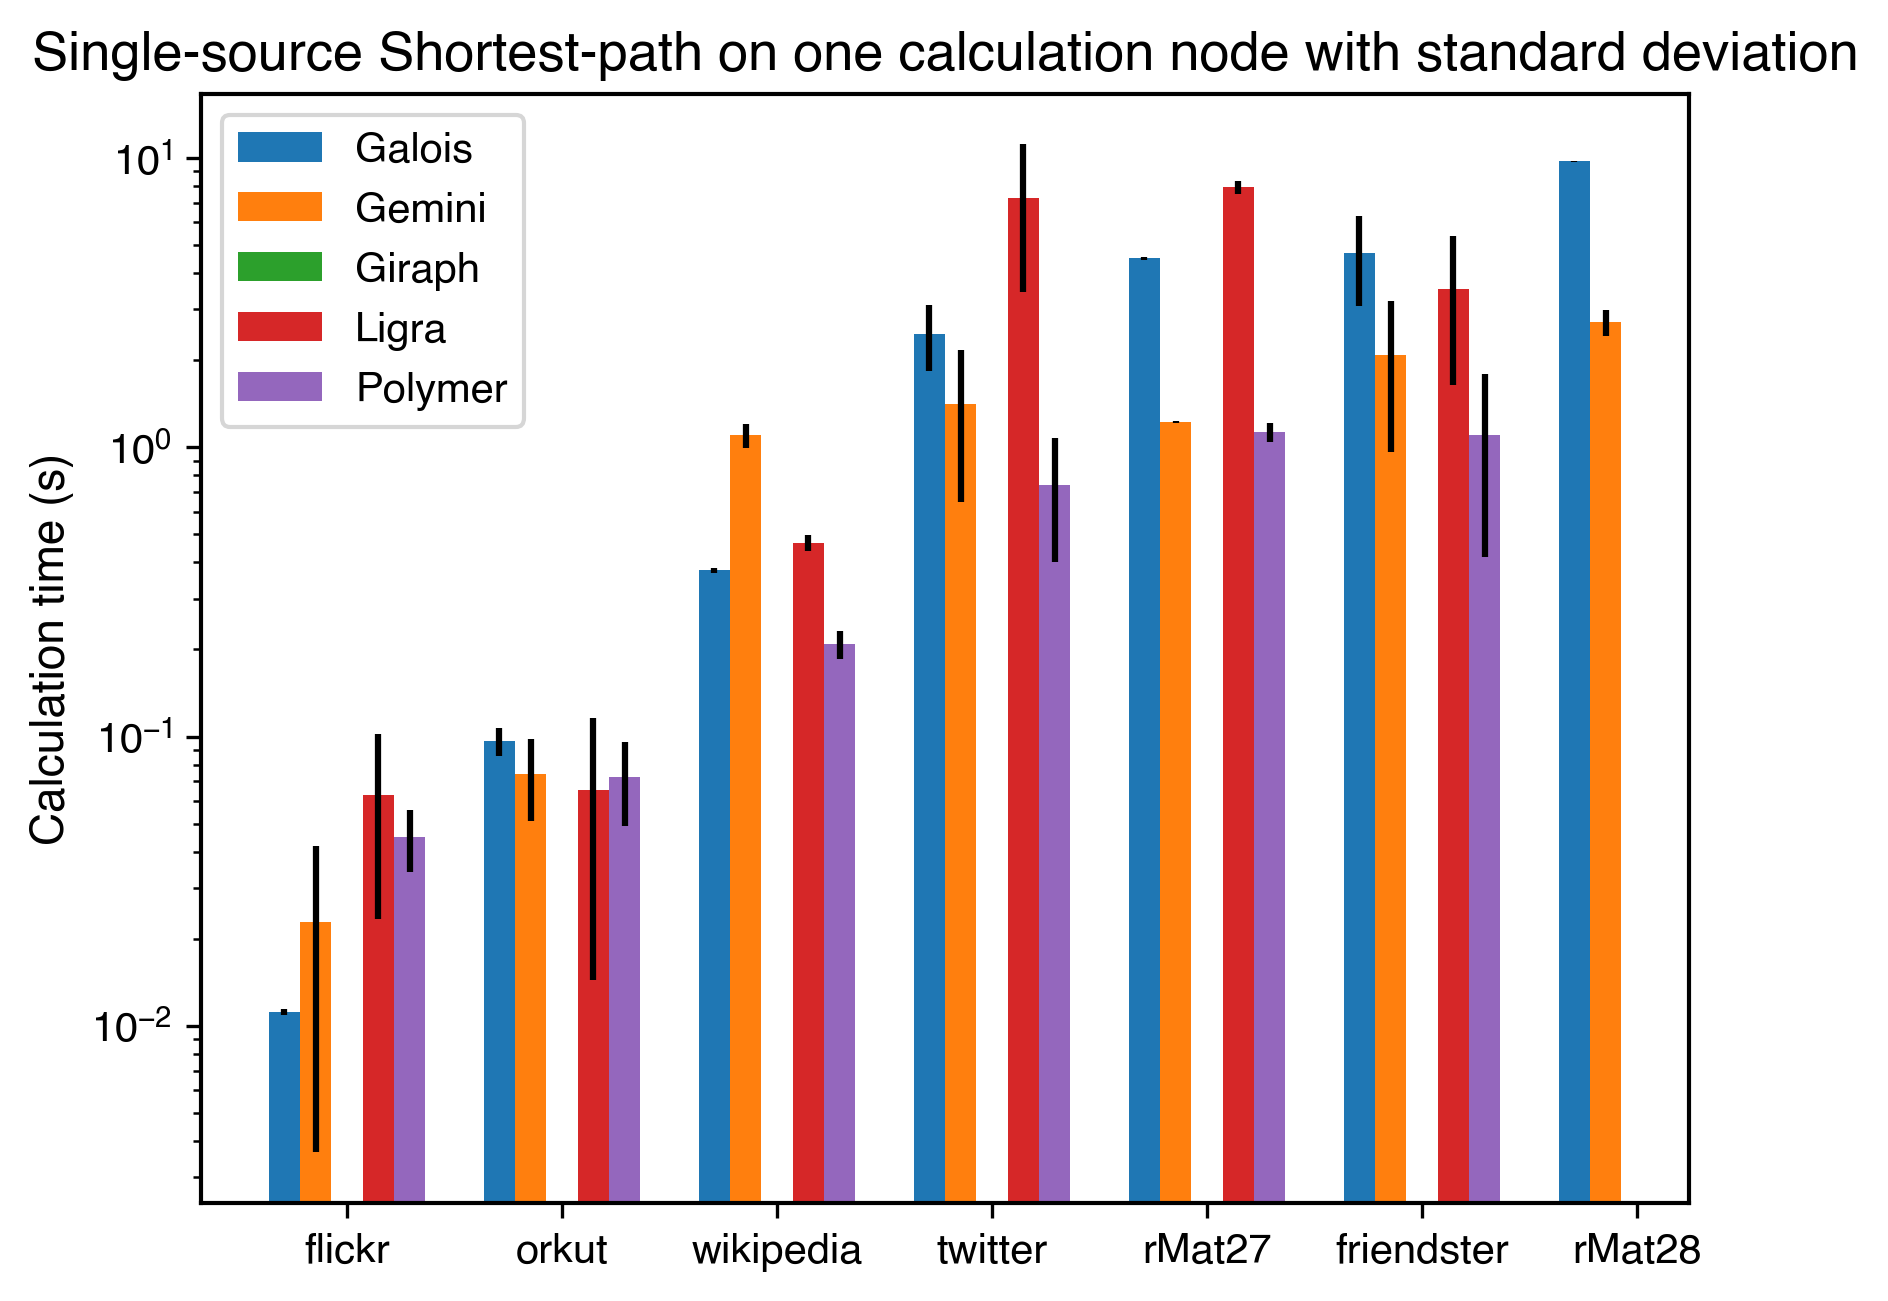
\includegraphics[width=\linewidth]{../../plots/singleNodeSSSP_calcTime.png}
		\caption{Calculation times for SSSP on a single node}
		\label{fig:singleNodeSSSP_calc}
	\end{subfigure}
	\hfil
	\begin{subfigure}{0.3\textwidth}
		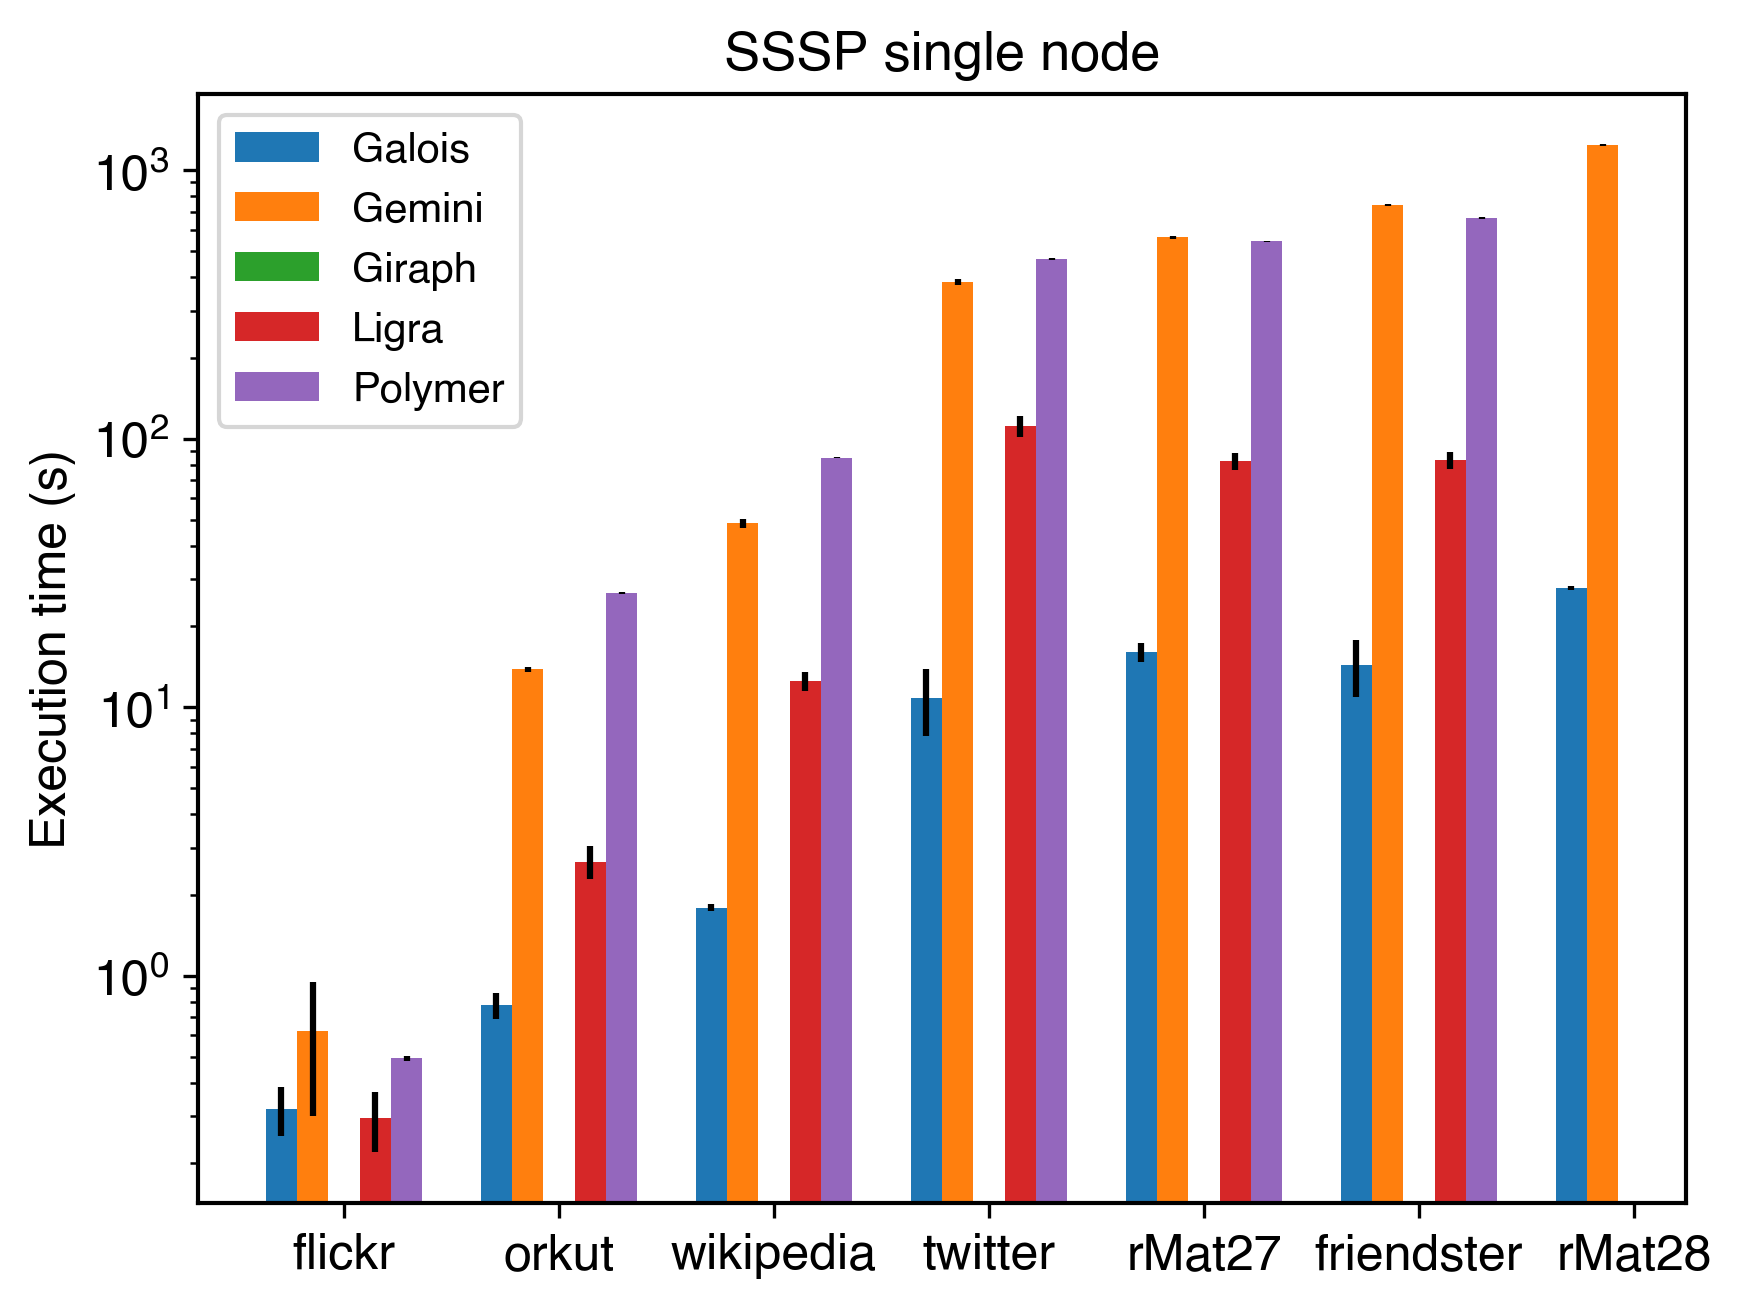
\includegraphics[width=\linewidth]{../../plots/singleNodeSSSP_execTime.png}
		\caption{Execution times for SSSP on a single node}
		\label{fig:singleNodeSSSP_exec}
	\end{subfigure}
	\hfil
	\begin{subfigure}{0.3\textwidth}
		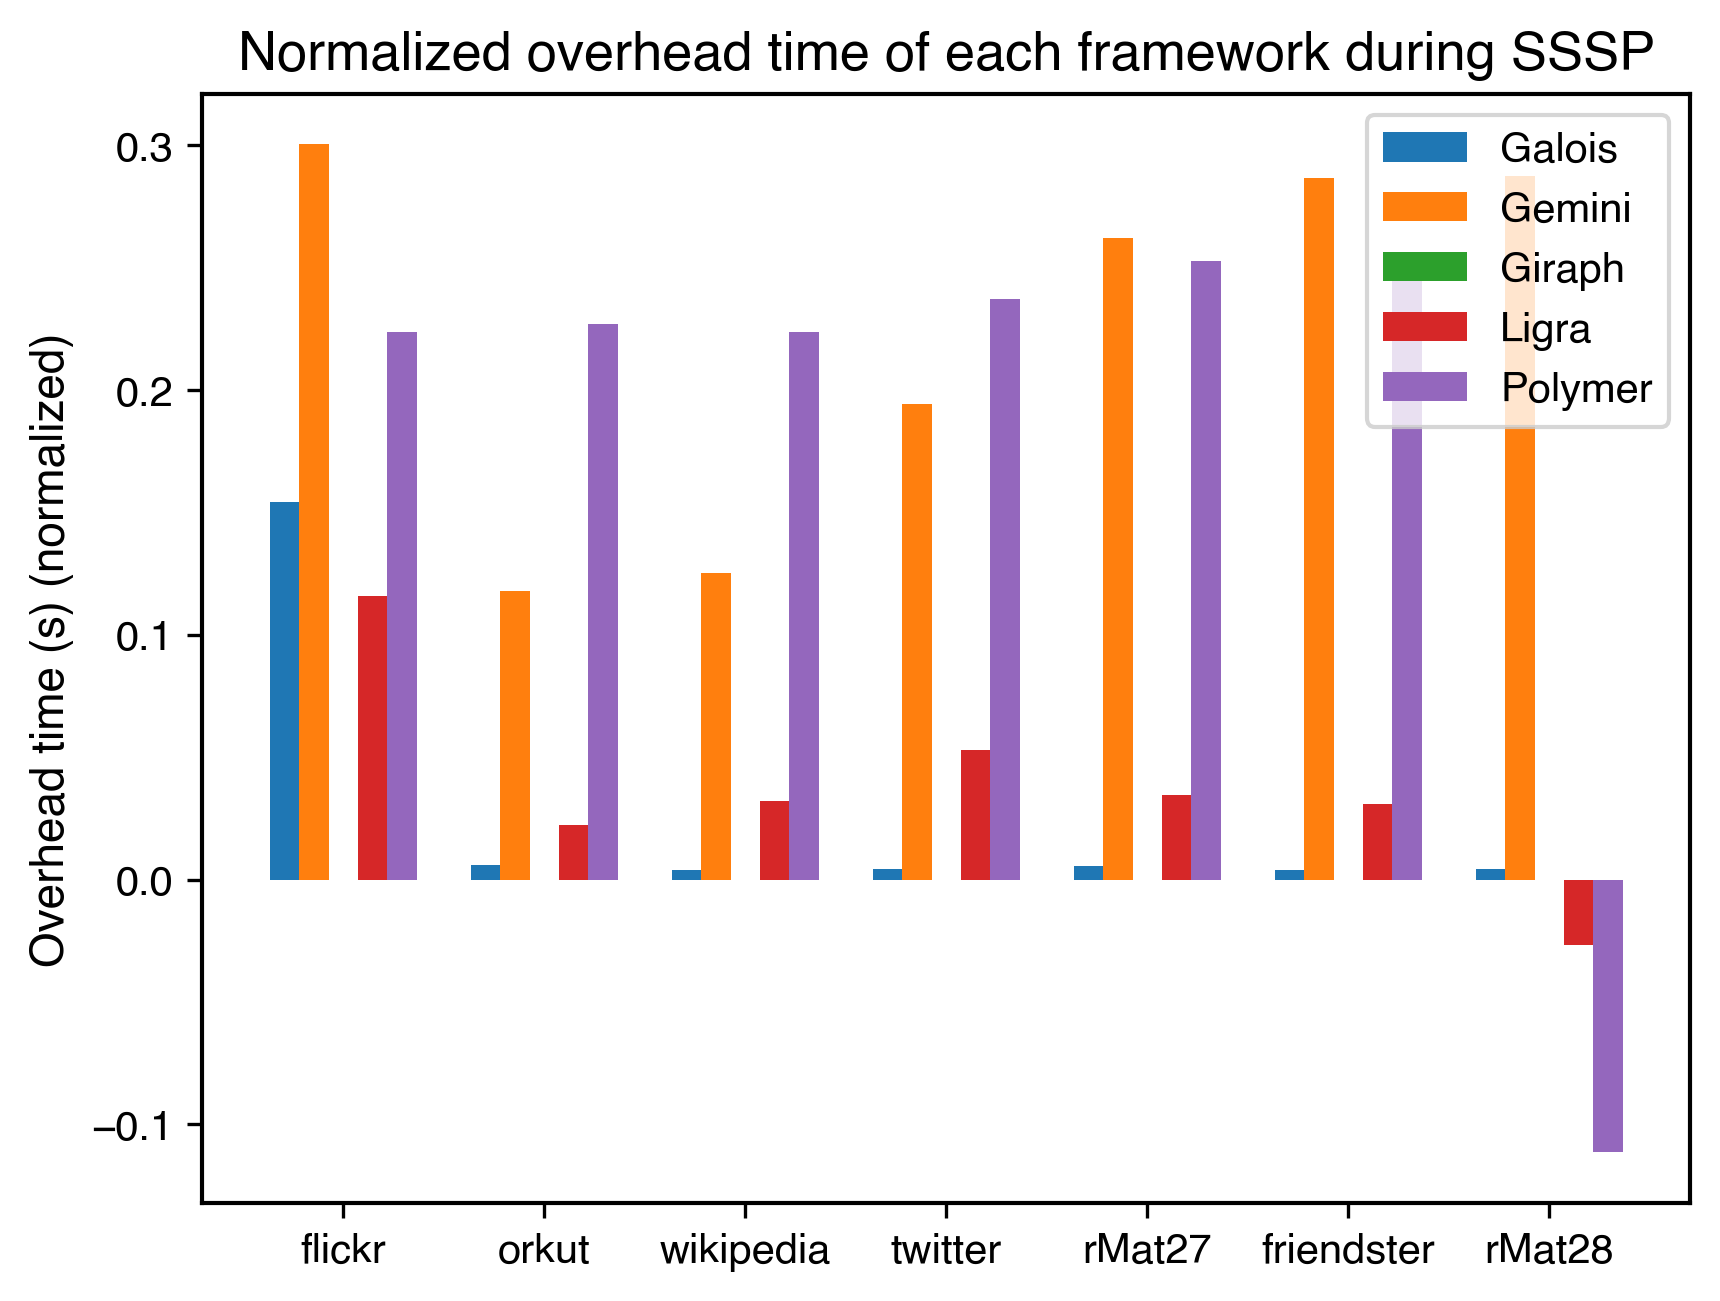
\includegraphics[width=\linewidth]{../../plots/singleNodeSSSP_overheadTimeNormalized.png}
		\caption{Overhead time normalized by the graph size in million edges}
		\label{fig:singleNodeSSSP_overheadNormalized}
	\end{subfigure}
	\caption{Average times on a single computation node, black bars represent one standard deviation in our testing.
	The runs on rMat28 for Ligra and Polymer failed and the frameworks were unable to complete the task.}
	\label{fig:singleNodeSSSP}
\end{figure*}








\subsubsection{Distributed}
\begin{figure}
	\begin{subfigure}{\columnwidth}
		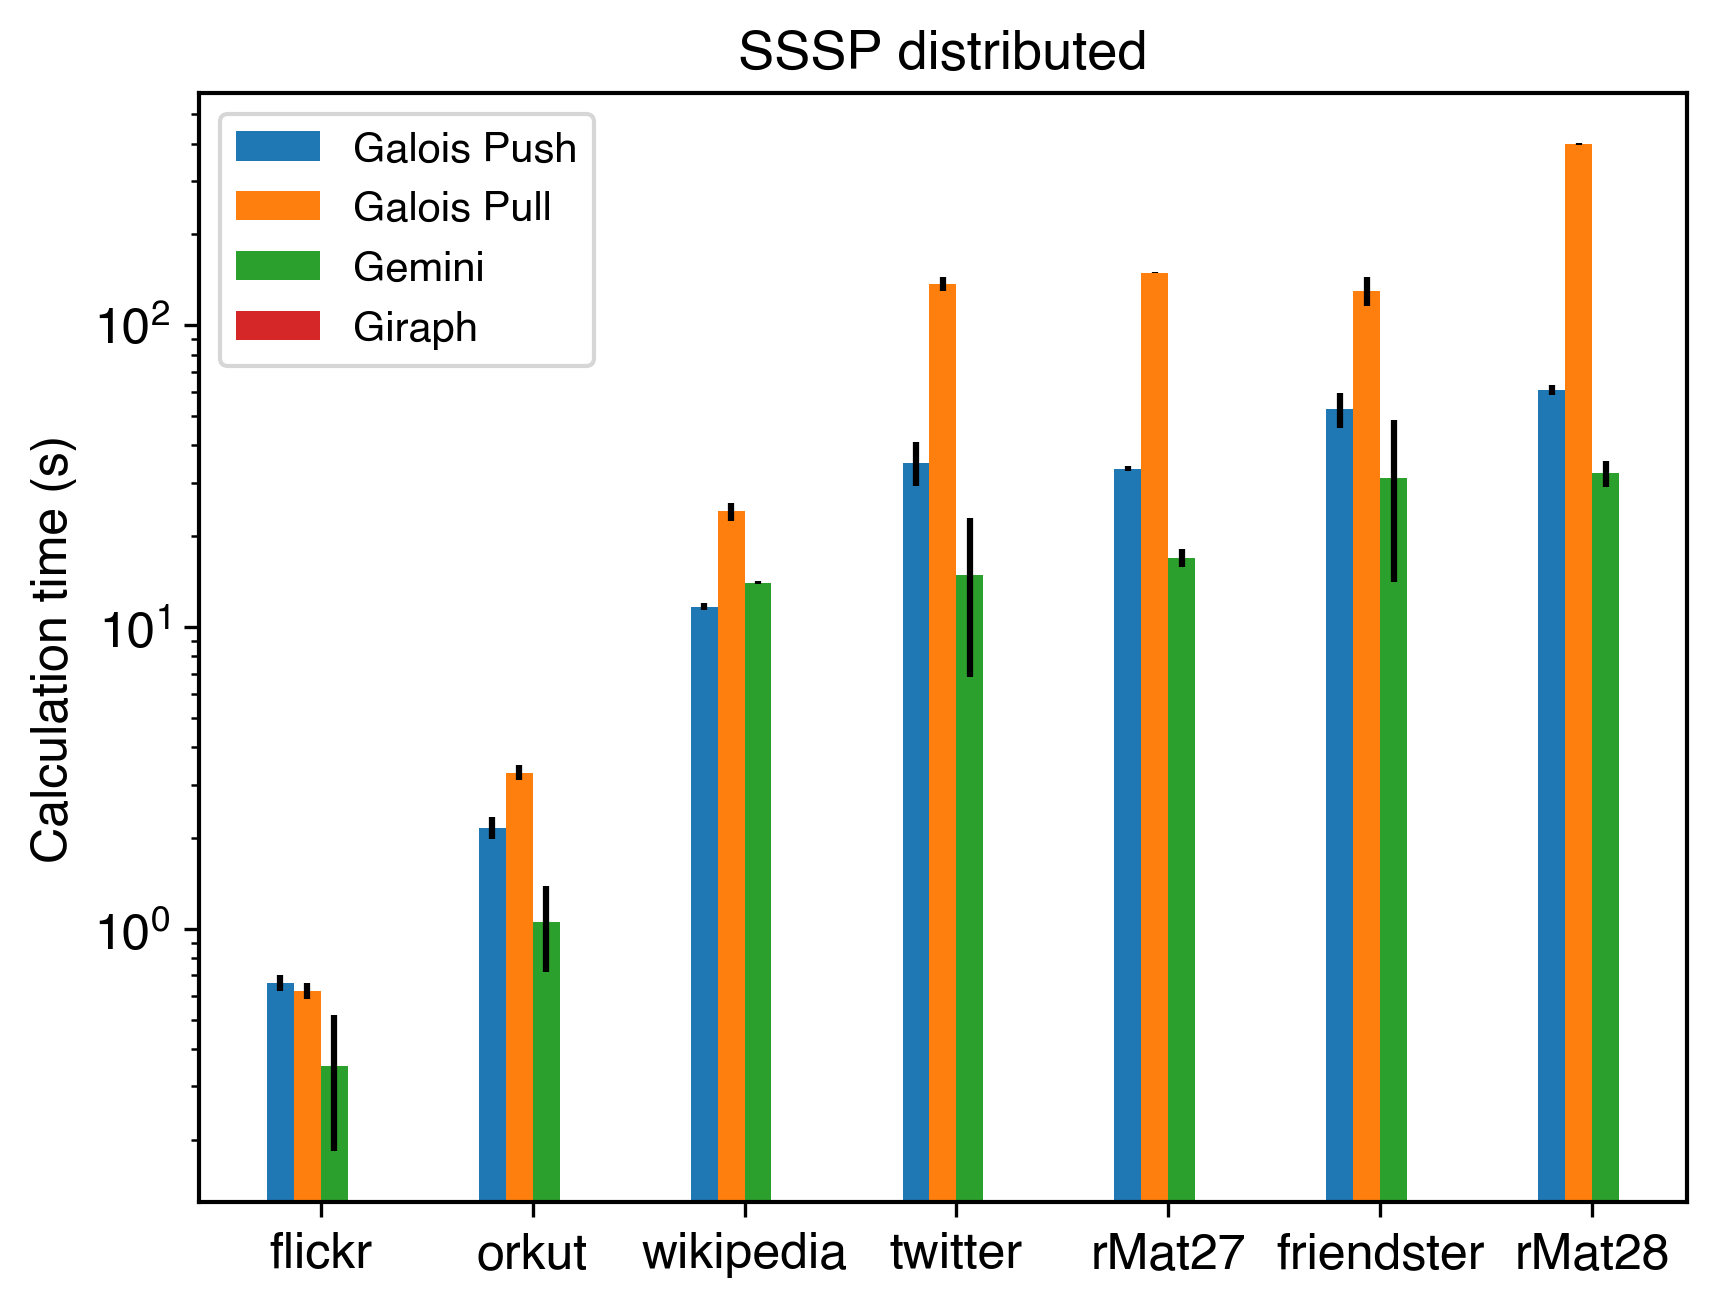
\includegraphics[width=\linewidth]{../../plots/distributedSSSP_calcTime.png}
		\caption{Calculation times for distributed SSSP}
		\label{fig:distributedSSSP_calc}
	\end{subfigure}
	\hfil
	\begin{subfigure}{\columnwidth}
		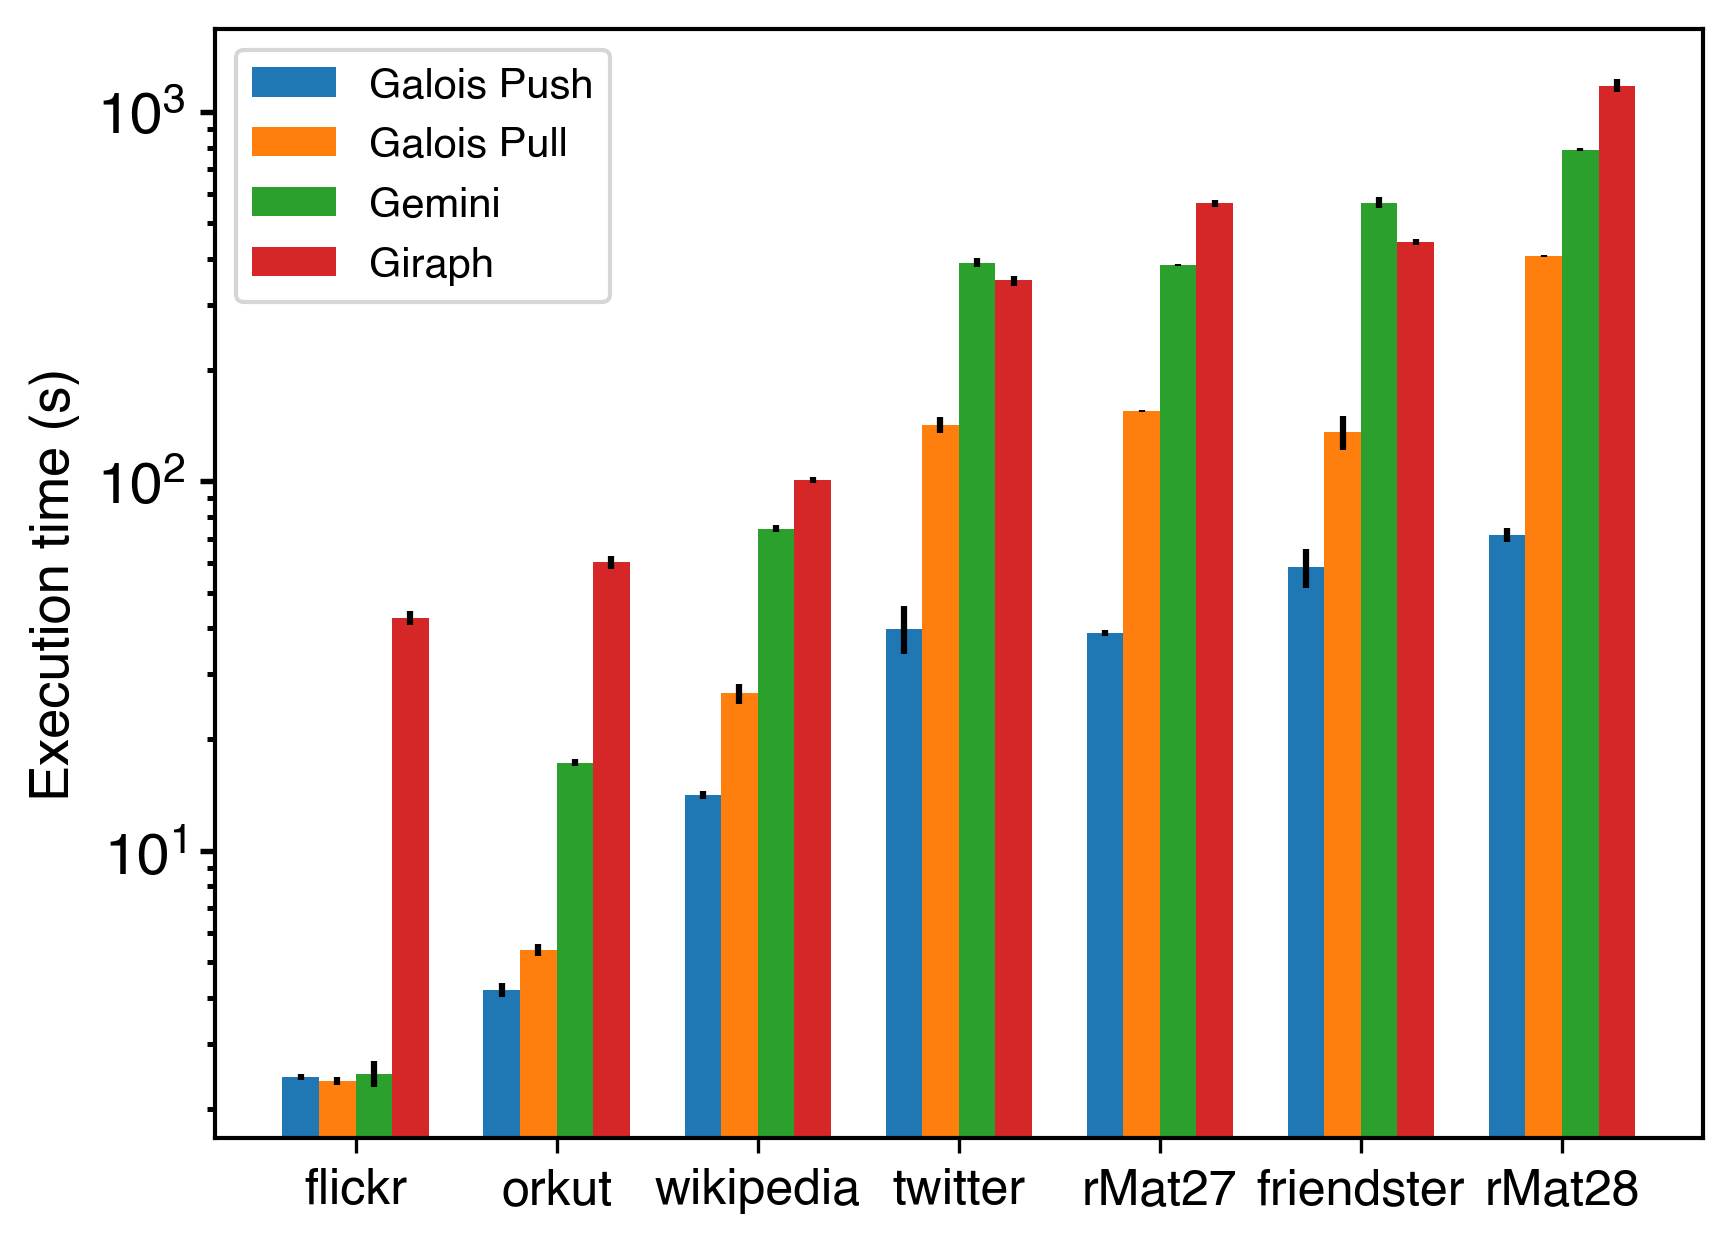
\includegraphics[width=\linewidth]{../../plots/distributedSSSP_execTime.png}
		\caption{Execution times for distributed SSSP}
		\label{fig:distributedSSSP_exec}
	\end{subfigure}
	\caption{Average times on the distributed cluster, black bars represent one standard deviation in our testing.}
	\label{fig:distributedSSSP}
\end{figure}

\begin{figure}
	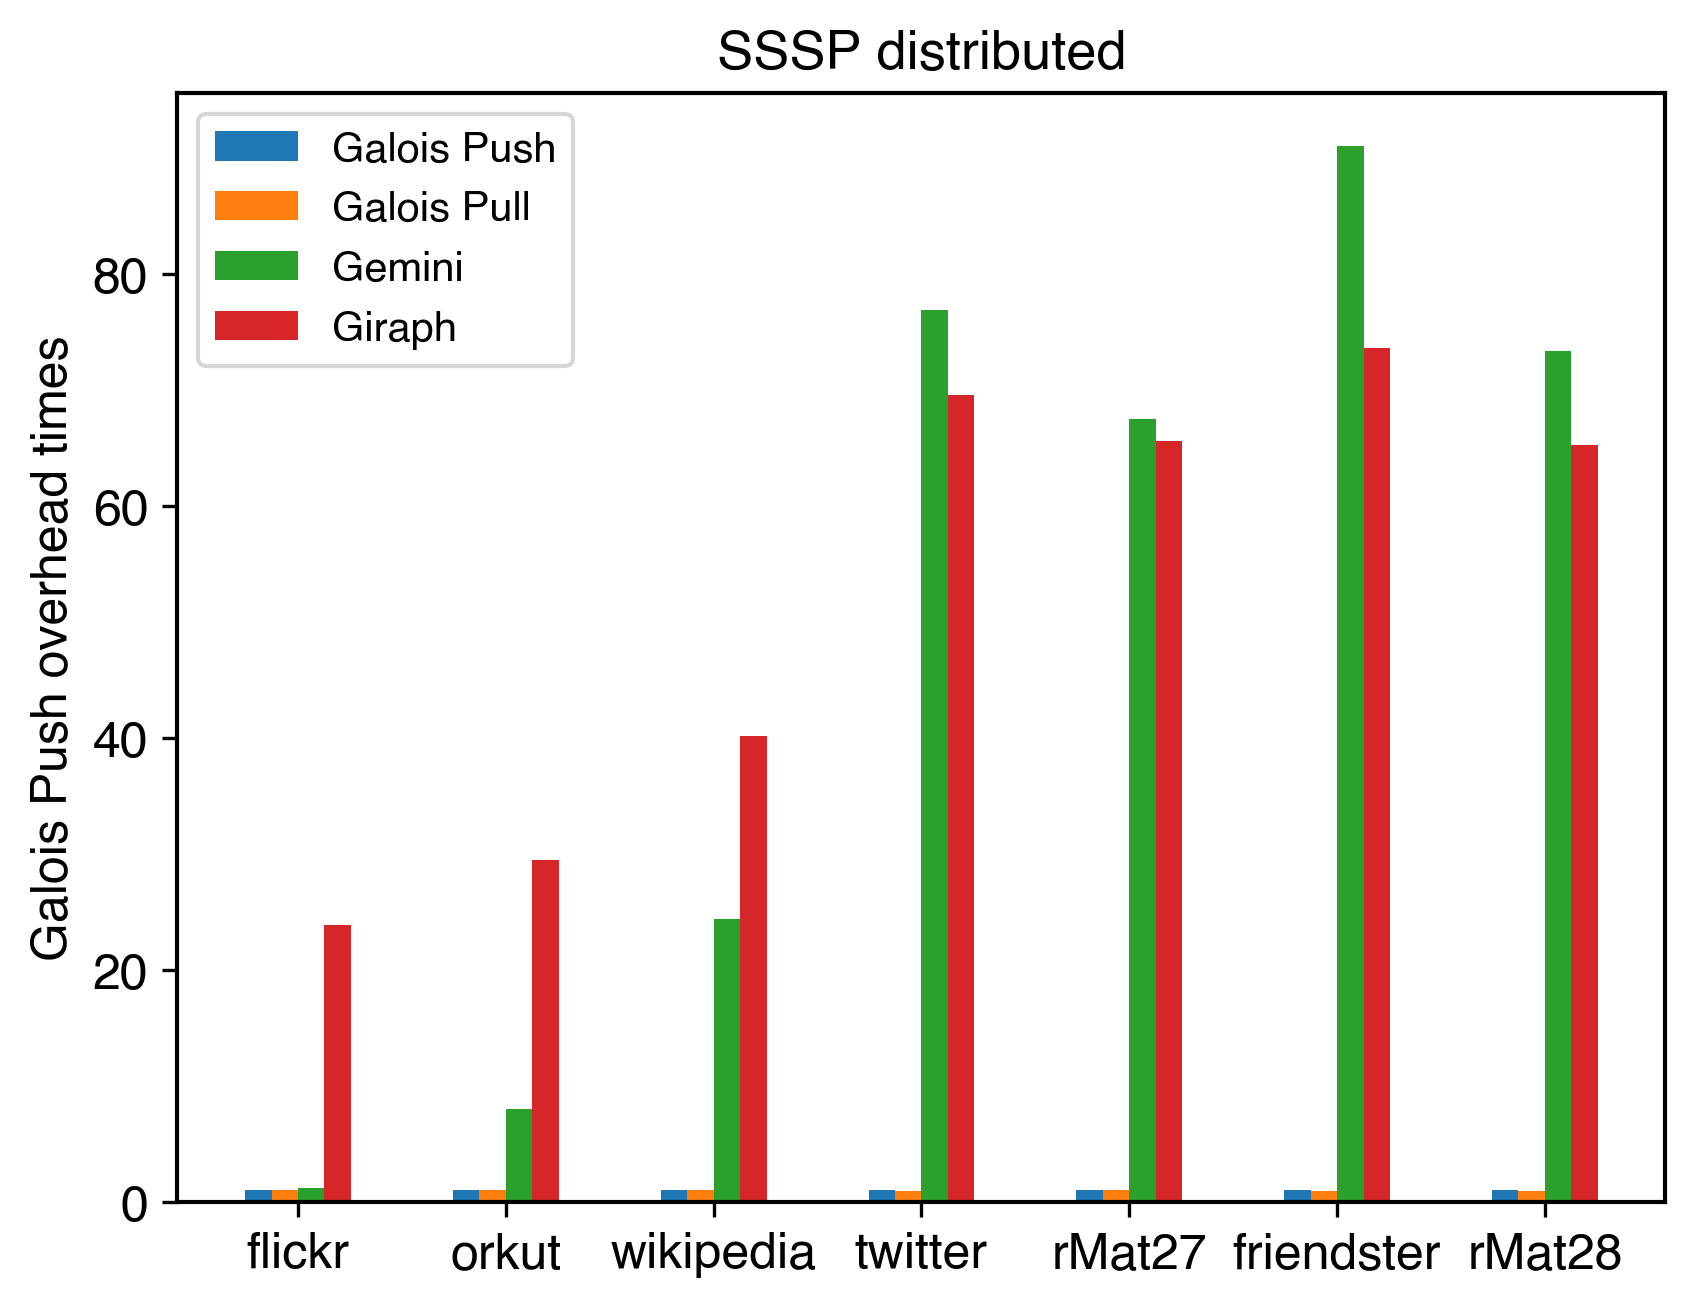
\includegraphics[width=\linewidth]{../../plots/distributedSSSP_overheadTimeNormalizedToGalois.png}
	\caption{Overhead times of each framework normalized by the overhead time of Galois Push}
	\label{fig:distributedSSSP_overhead}
\end{figure}

For the distributed scenario, \autoref{fig:distributedSSSP} shows the benchmark results as calculation and execution times. 

Results are especially interesting for Giraph since it seems to not cope well with synthetic graphs. Analyzing the computation times in \autoref{fig:distributedSSSP_calc}, we see that it is the fastest framework on our real-world graphs. And that with a considerable margin of other frameworks always taking at least 50\% longer (Gemini on flickr) up to Galois Pull needing 18$\times$ longer on wikipedia.  
On both synthetic graphs however, Giraph is the slowest to compute. Giraph requires 12$\times$ or even 15$\times$ the computation time of Gemini on rMat27 or rMat28 respectively.

While Giraph's computation times are very competitive, when comparing the execution times in \autoref{fig:distributedSSSP_exec} we see that Giraph is actually the slowest framework on 5 out of 7 graphs. For the other two, namely twitter and friendster, Giraph is second slowest with only Gemini taking longer to complete.

Giraph and Gemini's very long execution times are only due to their overhead being many orders of magnitude larger than Galois overhead (\autoref{fig:distributedSSSP_overhead}).
Overhead for Gemini is greater than that of Galois on every graph. From just a 20\% increase on flickr up to friendster, where the overhead is 90$\times$ that of Galois Push.
For Giraph the overhead times are not as extreme but still generally worse. Even on flickr, Giraph's overhead time is already 23$\times$ that of Galois. On friendster, where Gemini was worst, Giraph \emph{only} requires 73$\times$ the overhead time of Galois.






\subsection{Breadth-first search}
In these figures, Galois with 96 threads is shown. Again, we show the impact of Galois' thread count in \autoref{sec:galois_speedup}.
\begin{figure*}
	\begin{subfigure}{0.3\textwidth}
		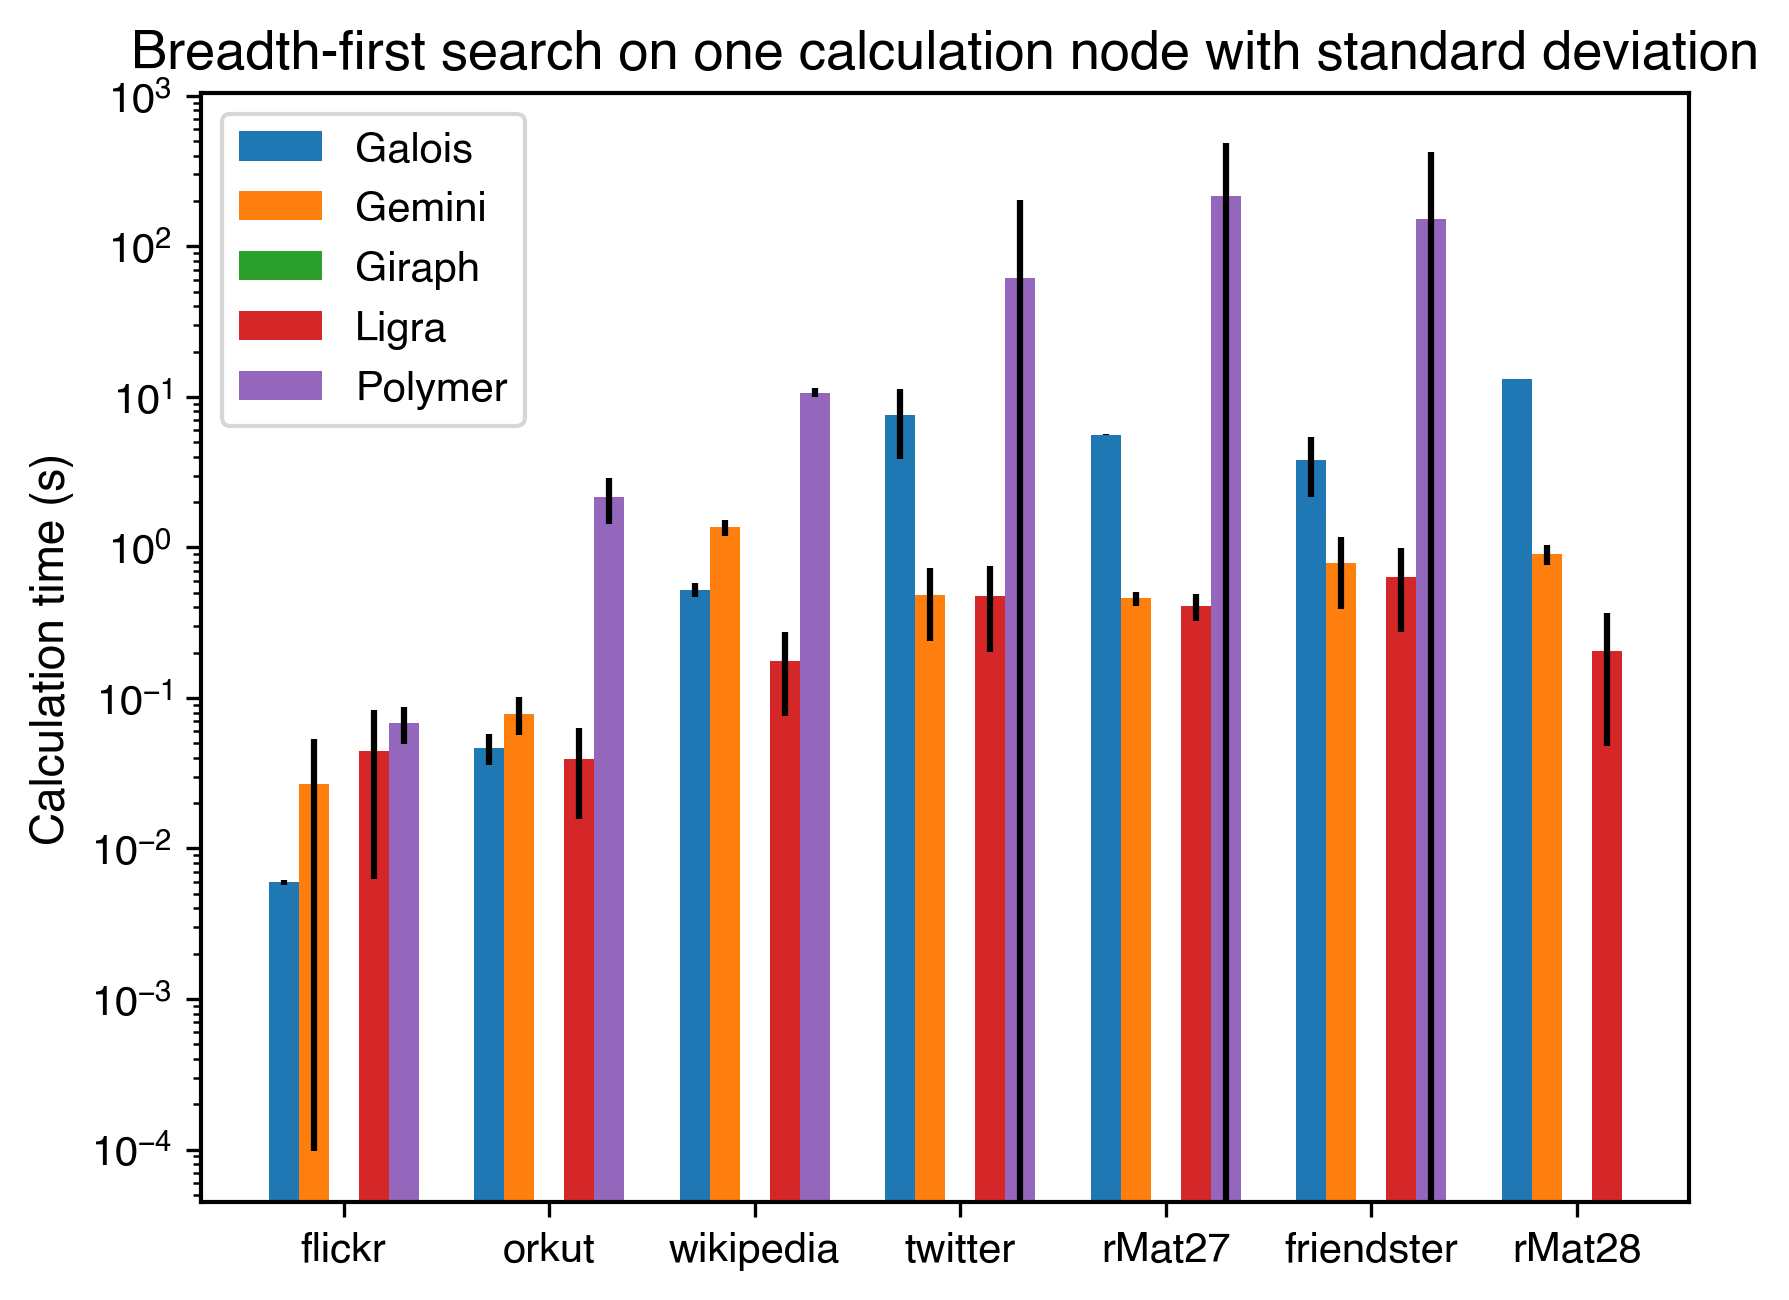
\includegraphics[width=\linewidth]{../../plots/singleNodeBFS_calcTime.png}
		\caption{Calculation times for BFS on a single node}
		\label{fig:singleNodeBFS_calc}
	\end{subfigure}
	\hfil
	\begin{subfigure}{0.3\textwidth}
		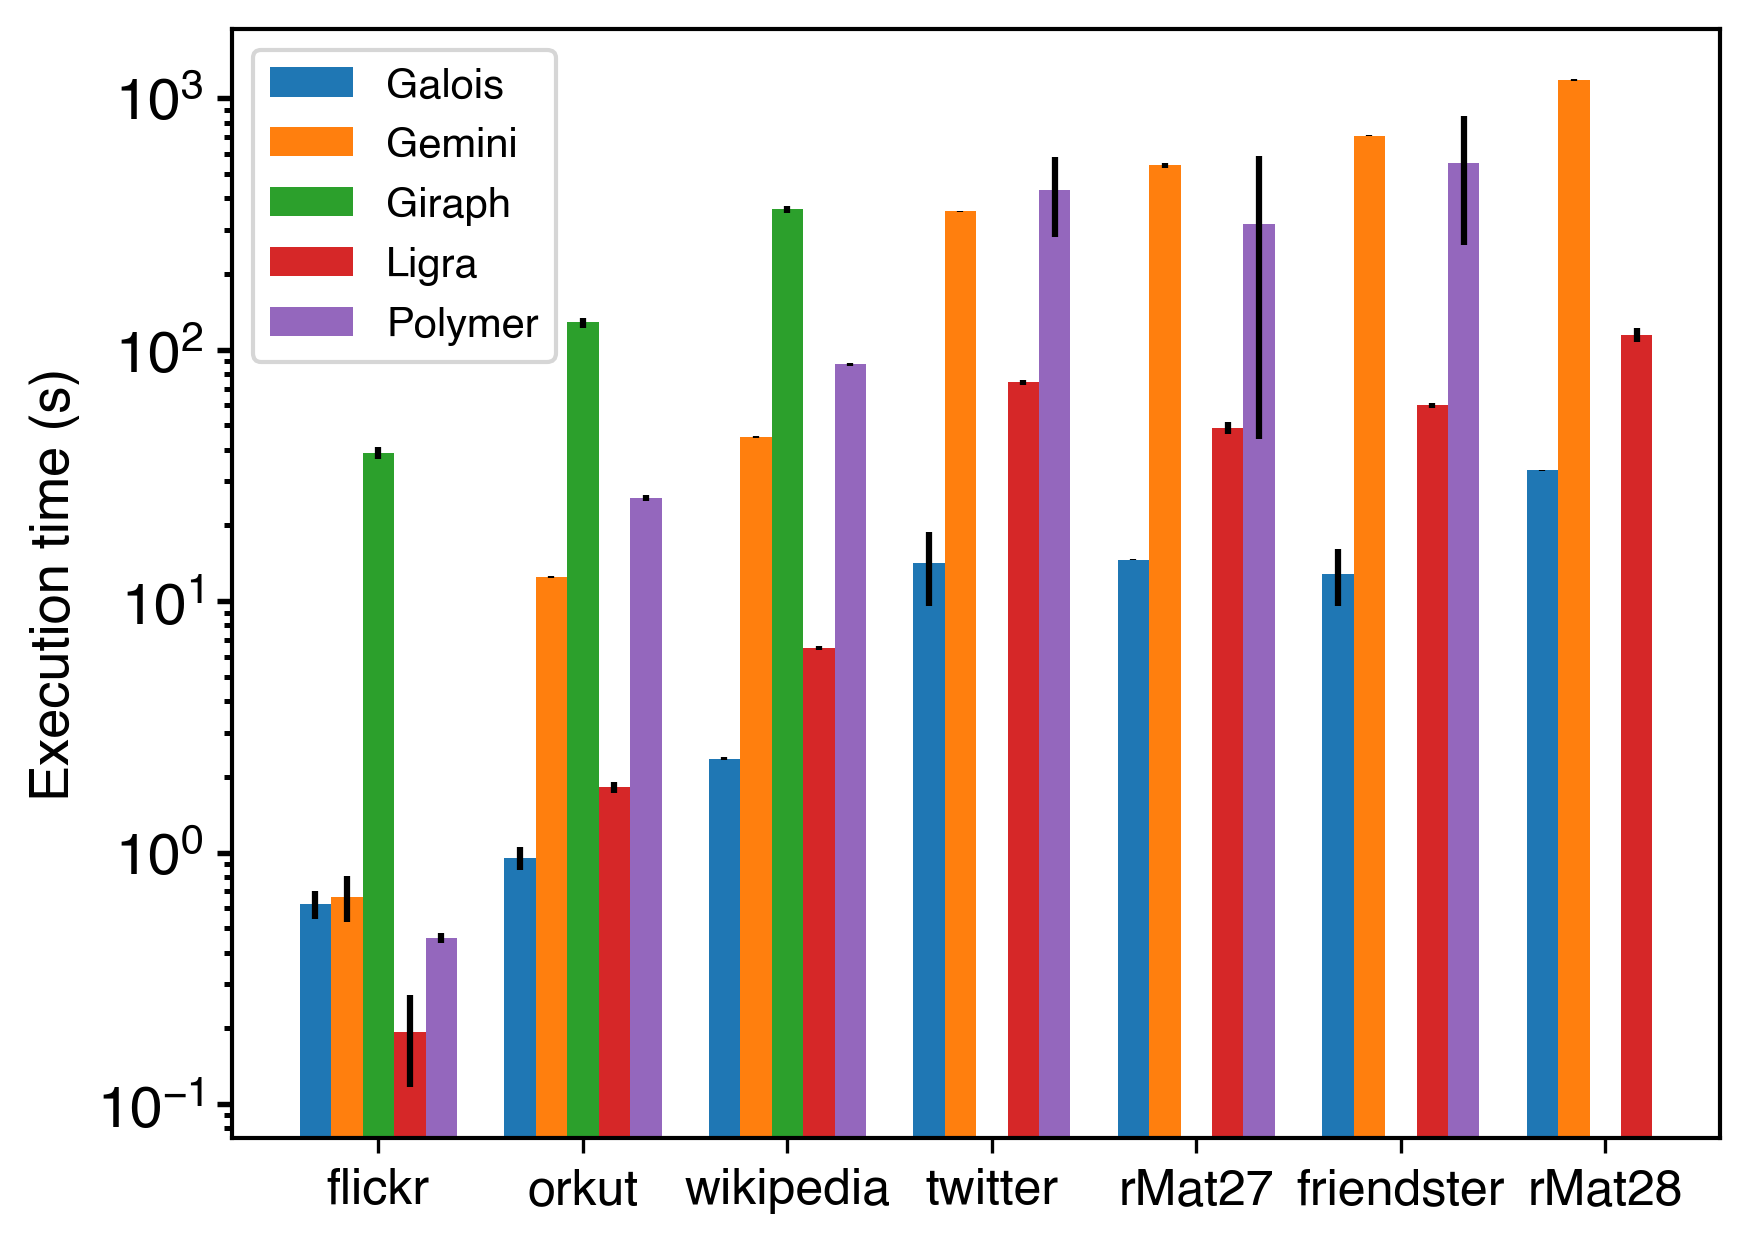
\includegraphics[width=\linewidth]{../../plots/singleNodeBFS_execTime.png}
		\caption{Execution times for BFS on a single node}
		\label{fig:singleNodeBFS_exec}
	\end{subfigure}
	\hfil
	\begin{subfigure}{0.3\textwidth}
		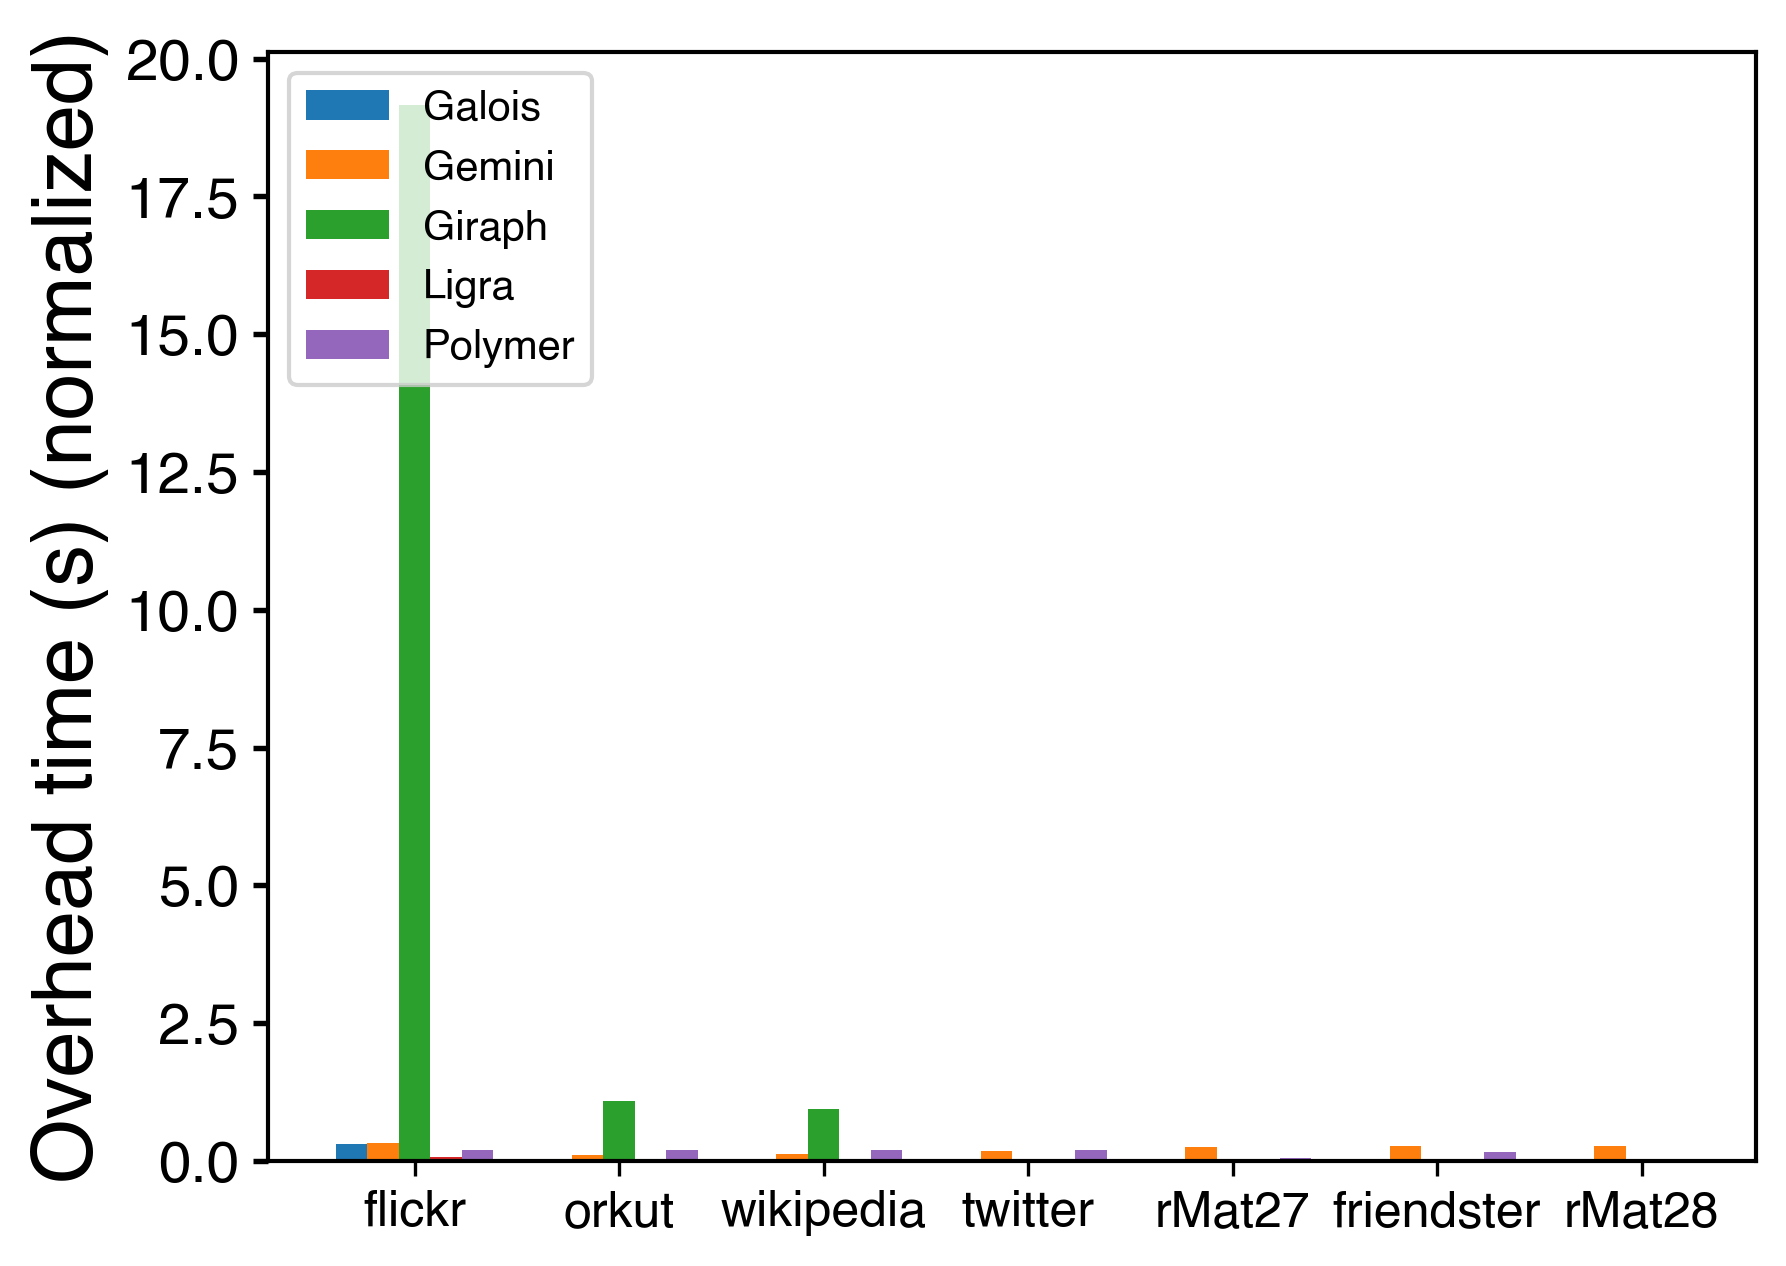
\includegraphics[width=\linewidth]{../../plots/singleNodeBFS_overheadTimeNormalized.png}
		\caption{Overhead time normalized by the graph size in million edges}
		\label{fig:singleNodeBFS_overheadNormalized}
	\end{subfigure}
	
	\caption{Average times on a single computation node, black bars represent one standard deviation in our testing}
\end{figure*}




\begin{figure*}
	\begin{subfigure}{0.3\textwidth}
		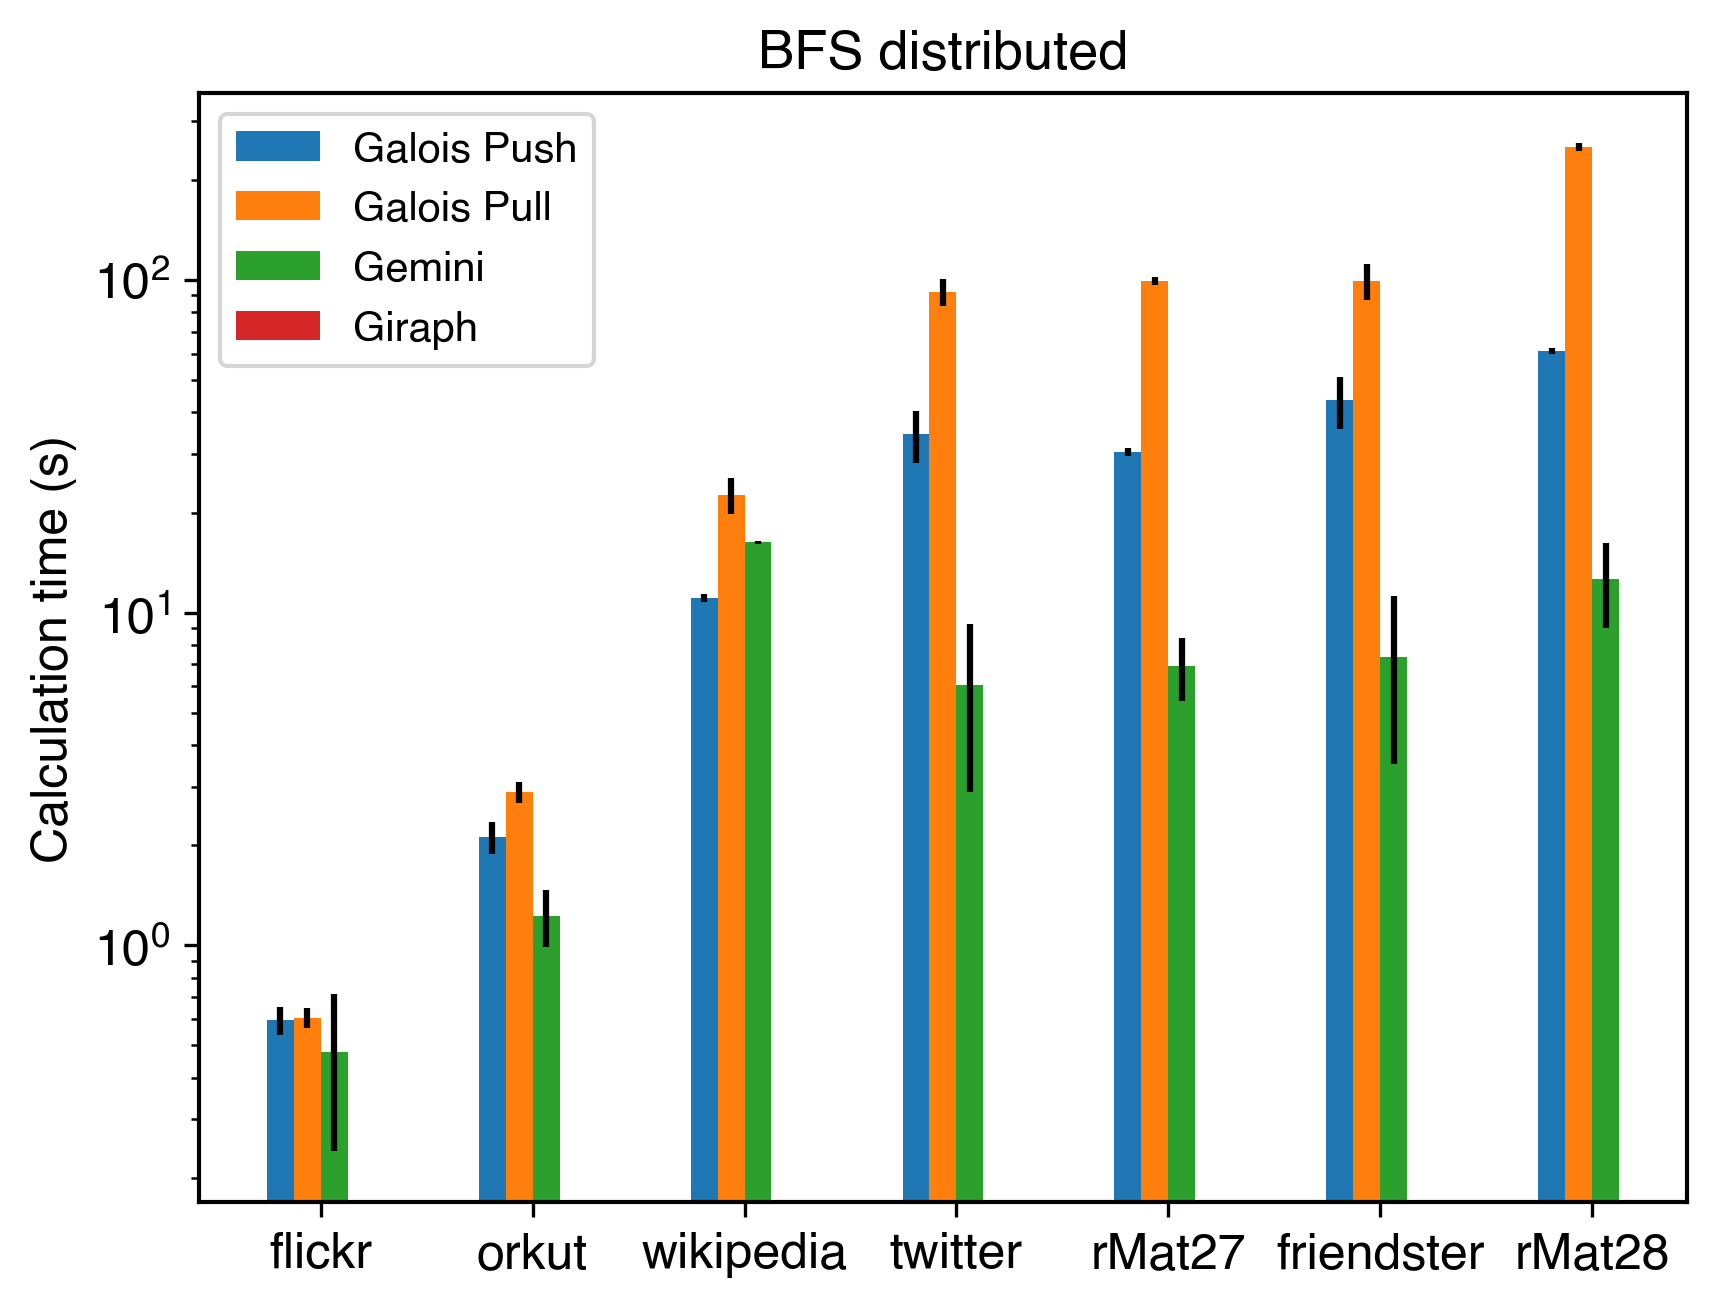
\includegraphics[width=\linewidth]{../../plots/distributedBFS_calcTime.png}
		\caption{Calculation times for distributed BFS}
		\label{fig:distributedBFS_calc}
	\end{subfigure}
	\hfil
	\begin{subfigure}{0.3\textwidth}
		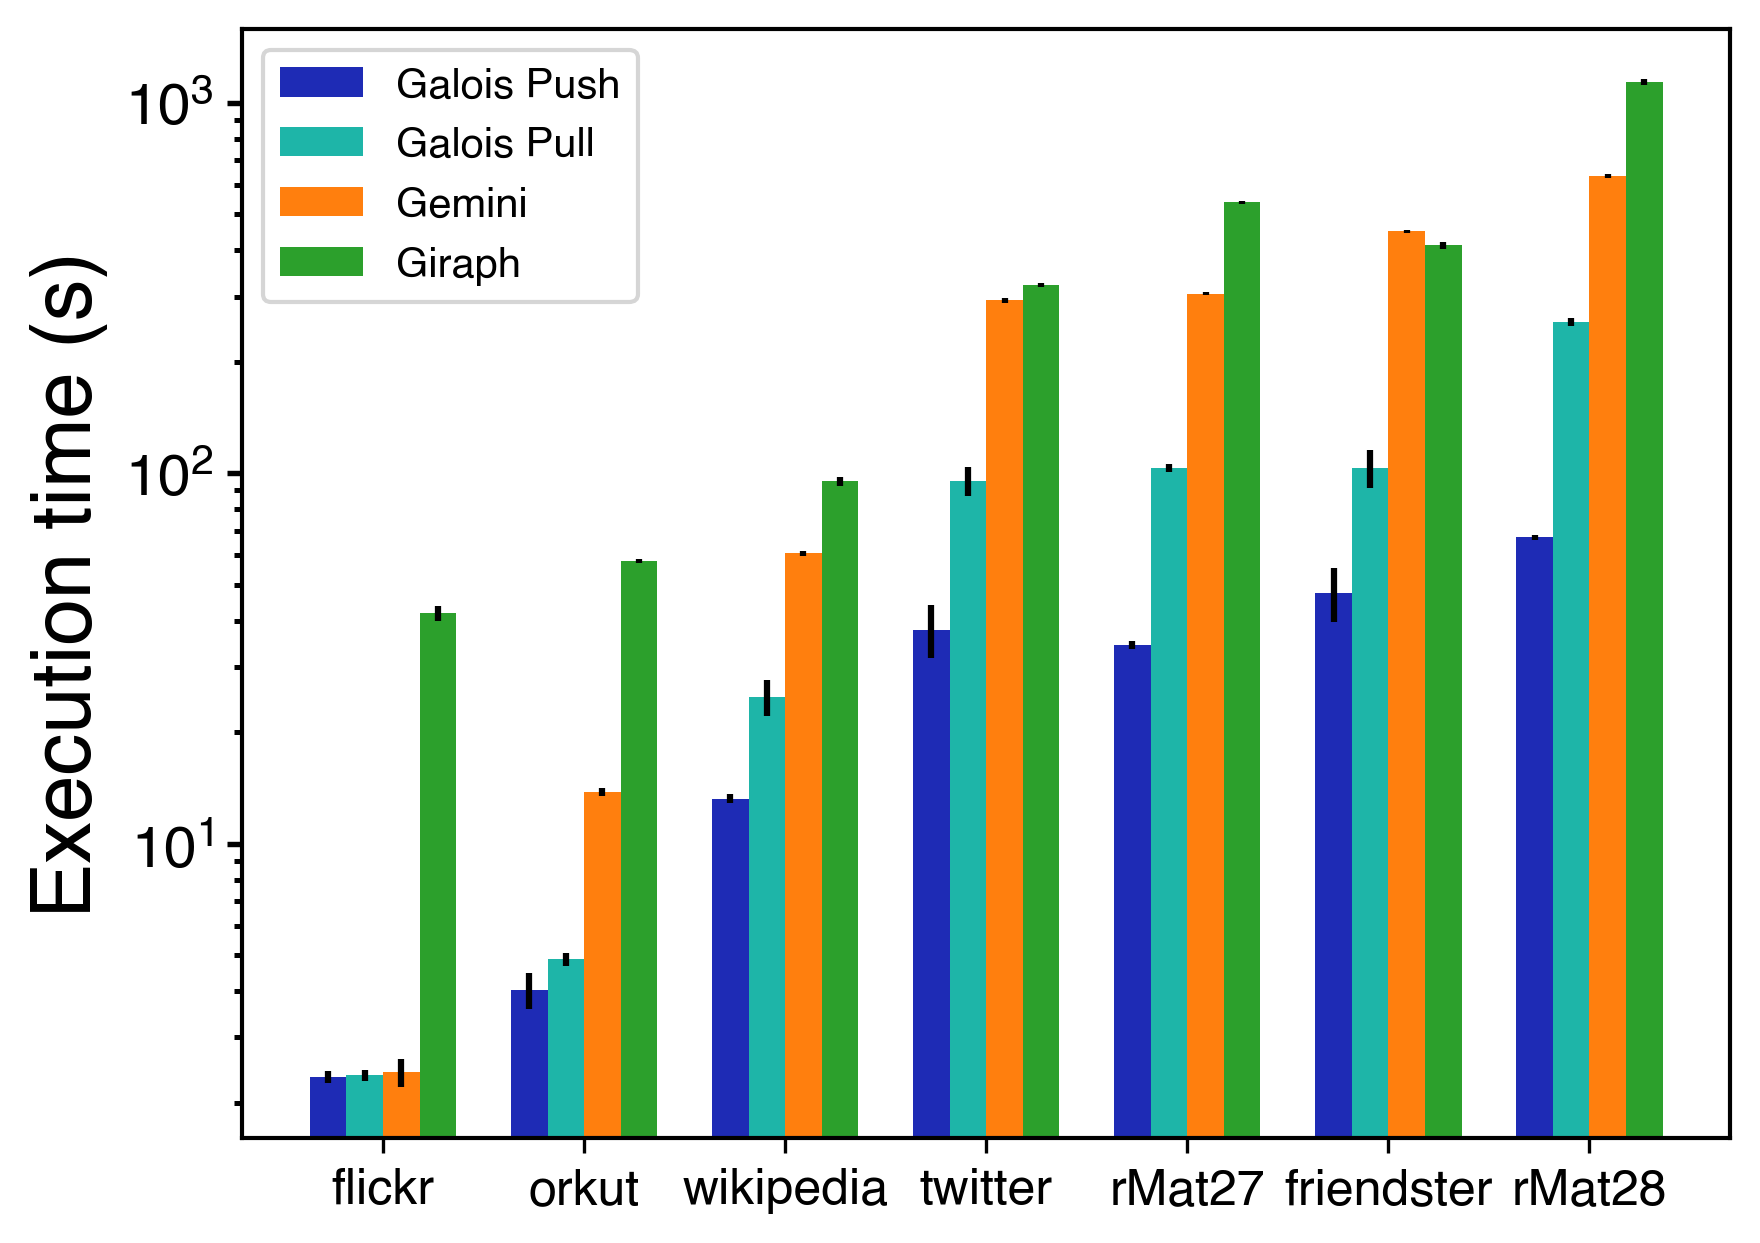
\includegraphics[width=\linewidth]{../../plots/distributedBFS_execTime.png}
		\caption{Execution times for distributed BFS}
		\label{fig:distributedBFS_exec}
	\end{subfigure}
	\hfil
	\begin{subfigure}{0.3\textwidth}
		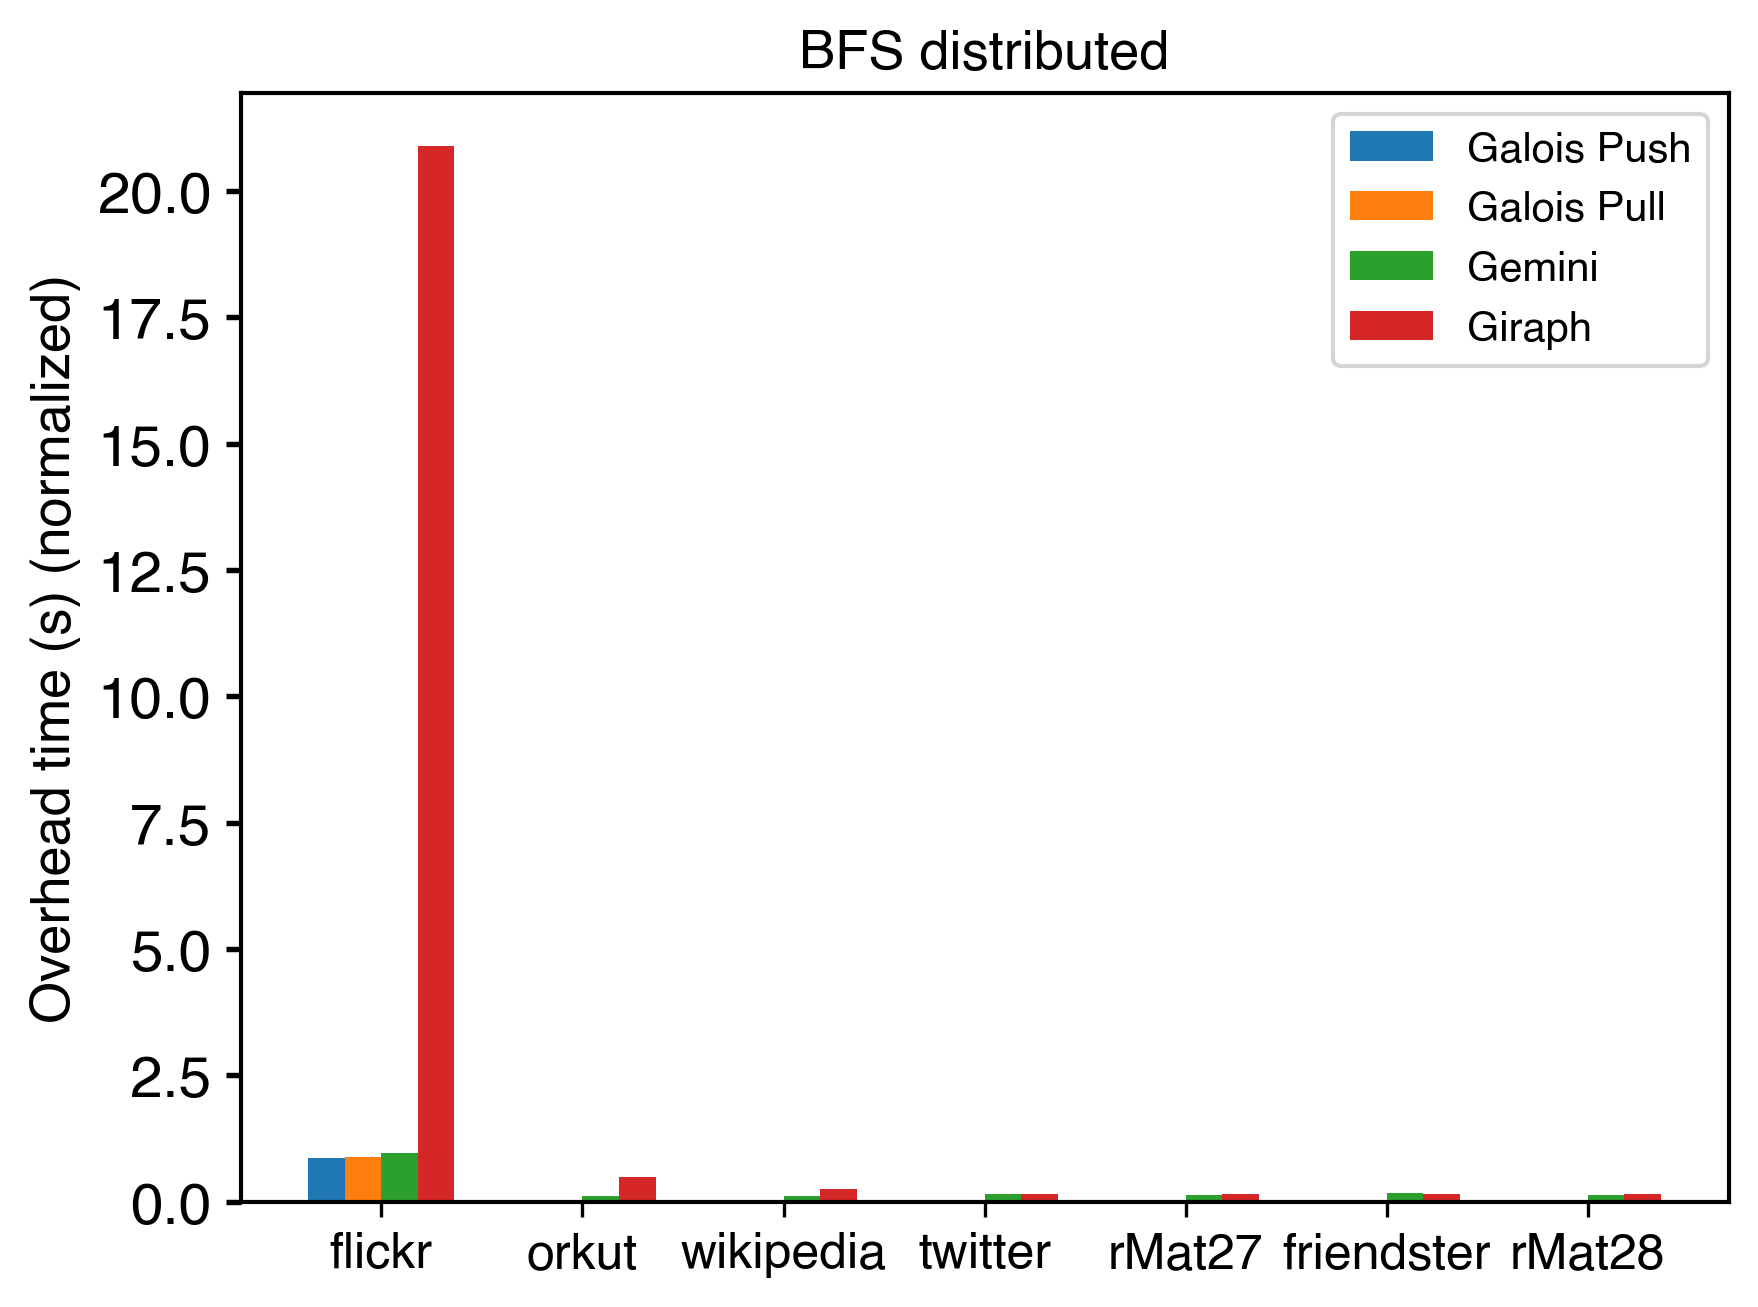
\includegraphics[width=\linewidth]{../../plots/distributedBFS_overheadTimeNormalized.png}
		\caption{Overhead time normalized by the graph size in million edges}
		\label{fig:distributedBFS_overheadNormalized}
	\end{subfigure}
	
	\caption{Average times on the distributed cluster, black bars represent one standard deviation in our testing}
\end{figure*}



\subsection{PageRank}

\begin{figure*}
	\begin{subfigure}{0.3\textwidth}
		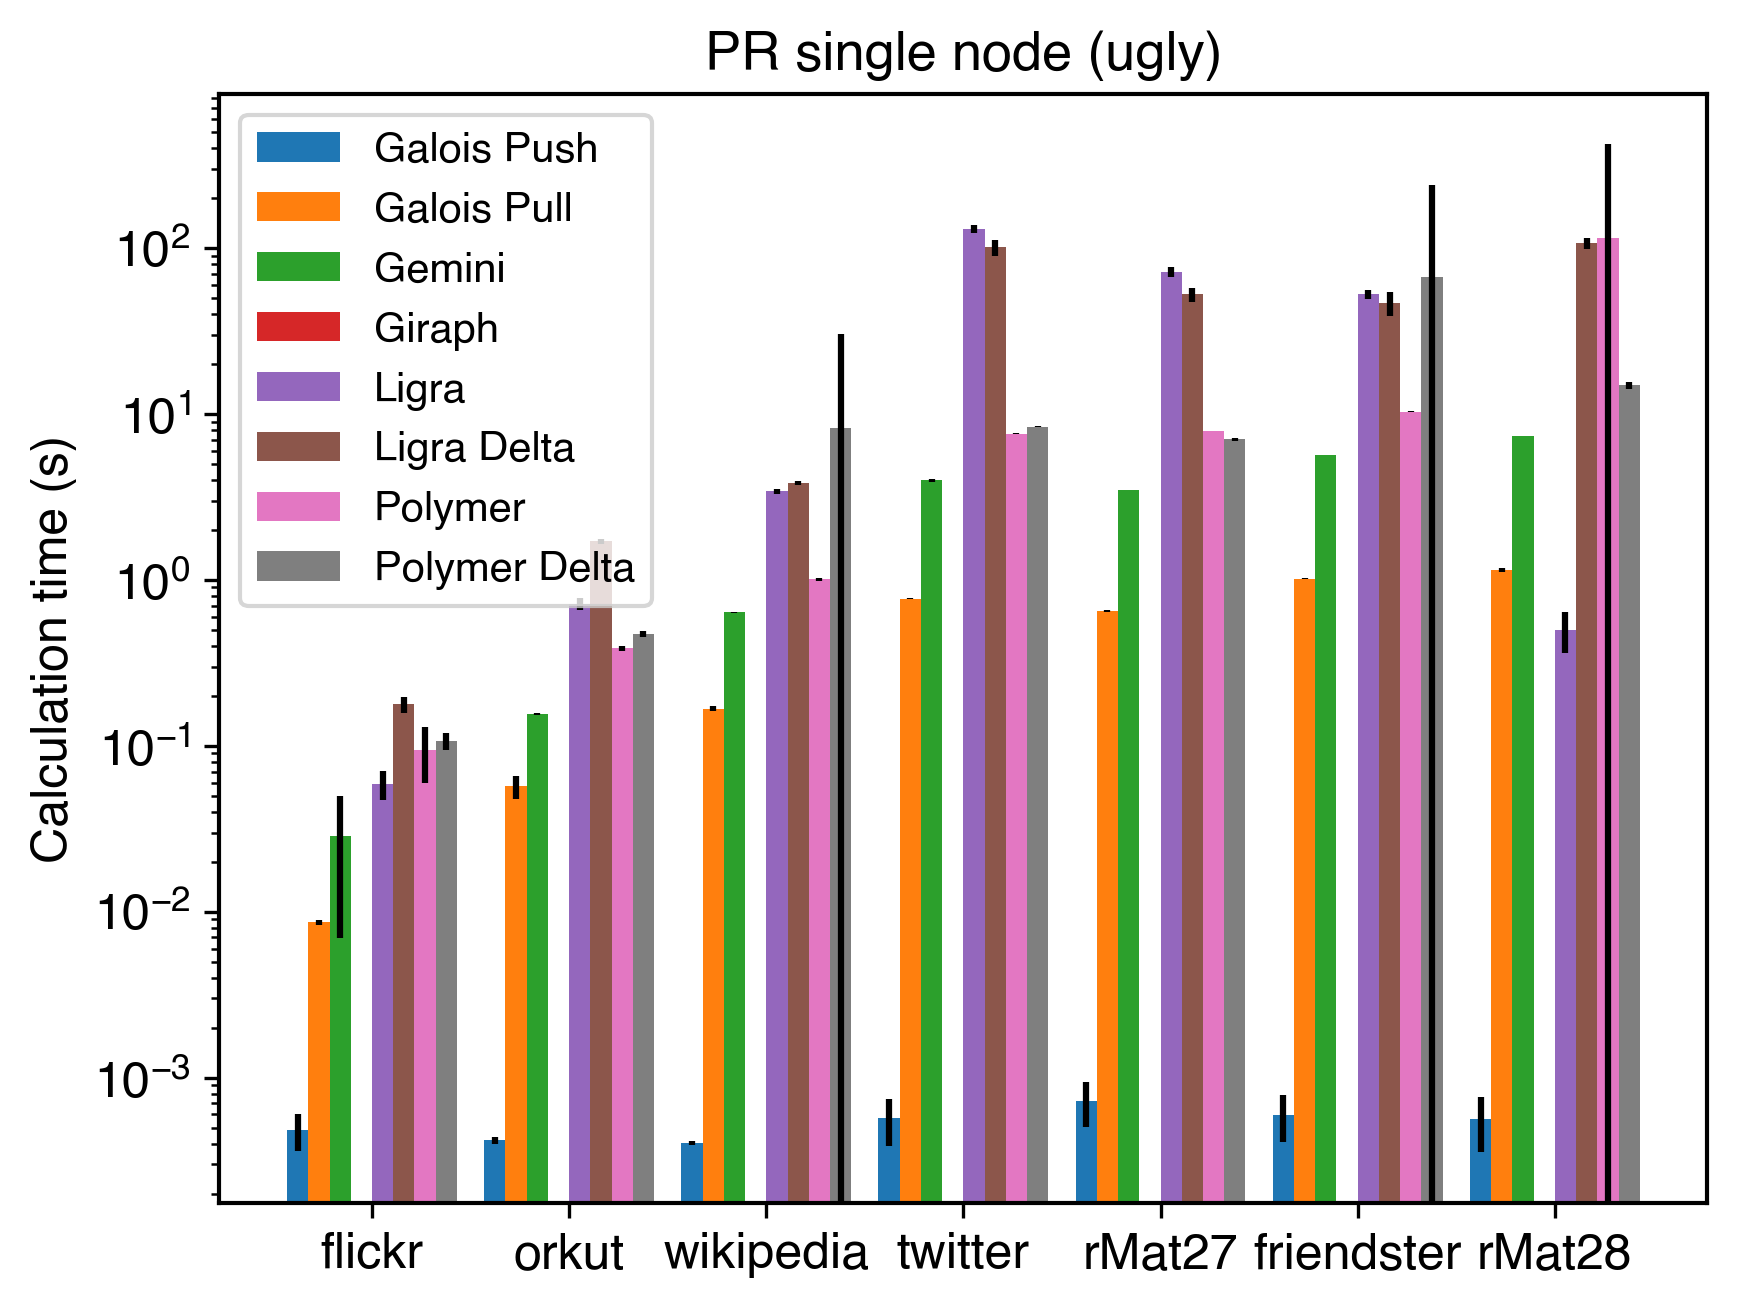
\includegraphics[width=\linewidth]{../../plots/singleNodePR_calcTime.png}
		\caption{Calculation times for PR on a single node}
		\label{fig:singleNodePR_calc}
	\end{subfigure}
	\hfil
	\begin{subfigure}{0.3\textwidth}
		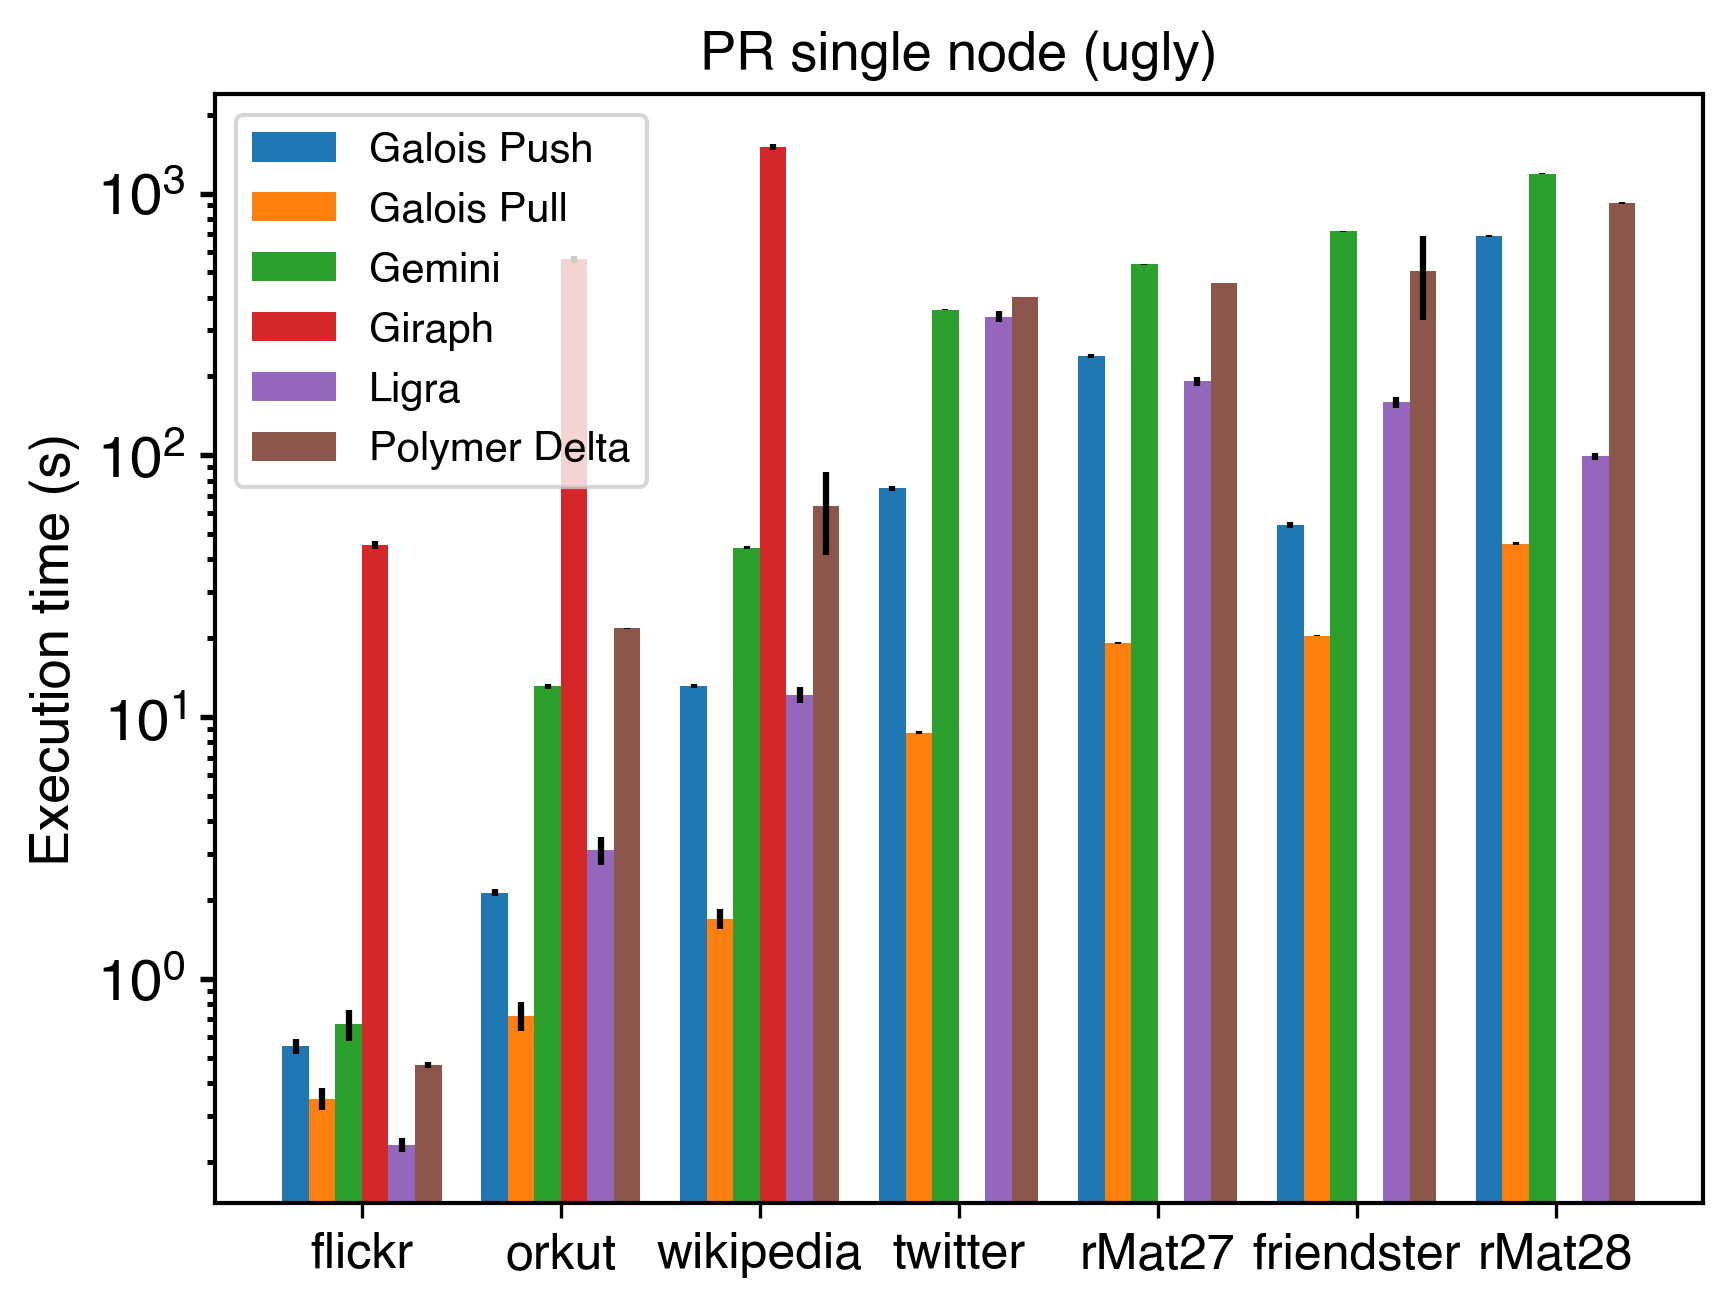
\includegraphics[width=\linewidth]{../../plots/singleNodePR_execTime.png}
		\caption{Execution times for PR on a single node}
		\label{fig:singleNodePR_exec}
	\end{subfigure}
	\hfil
	\begin{subfigure}{0.3\textwidth}
		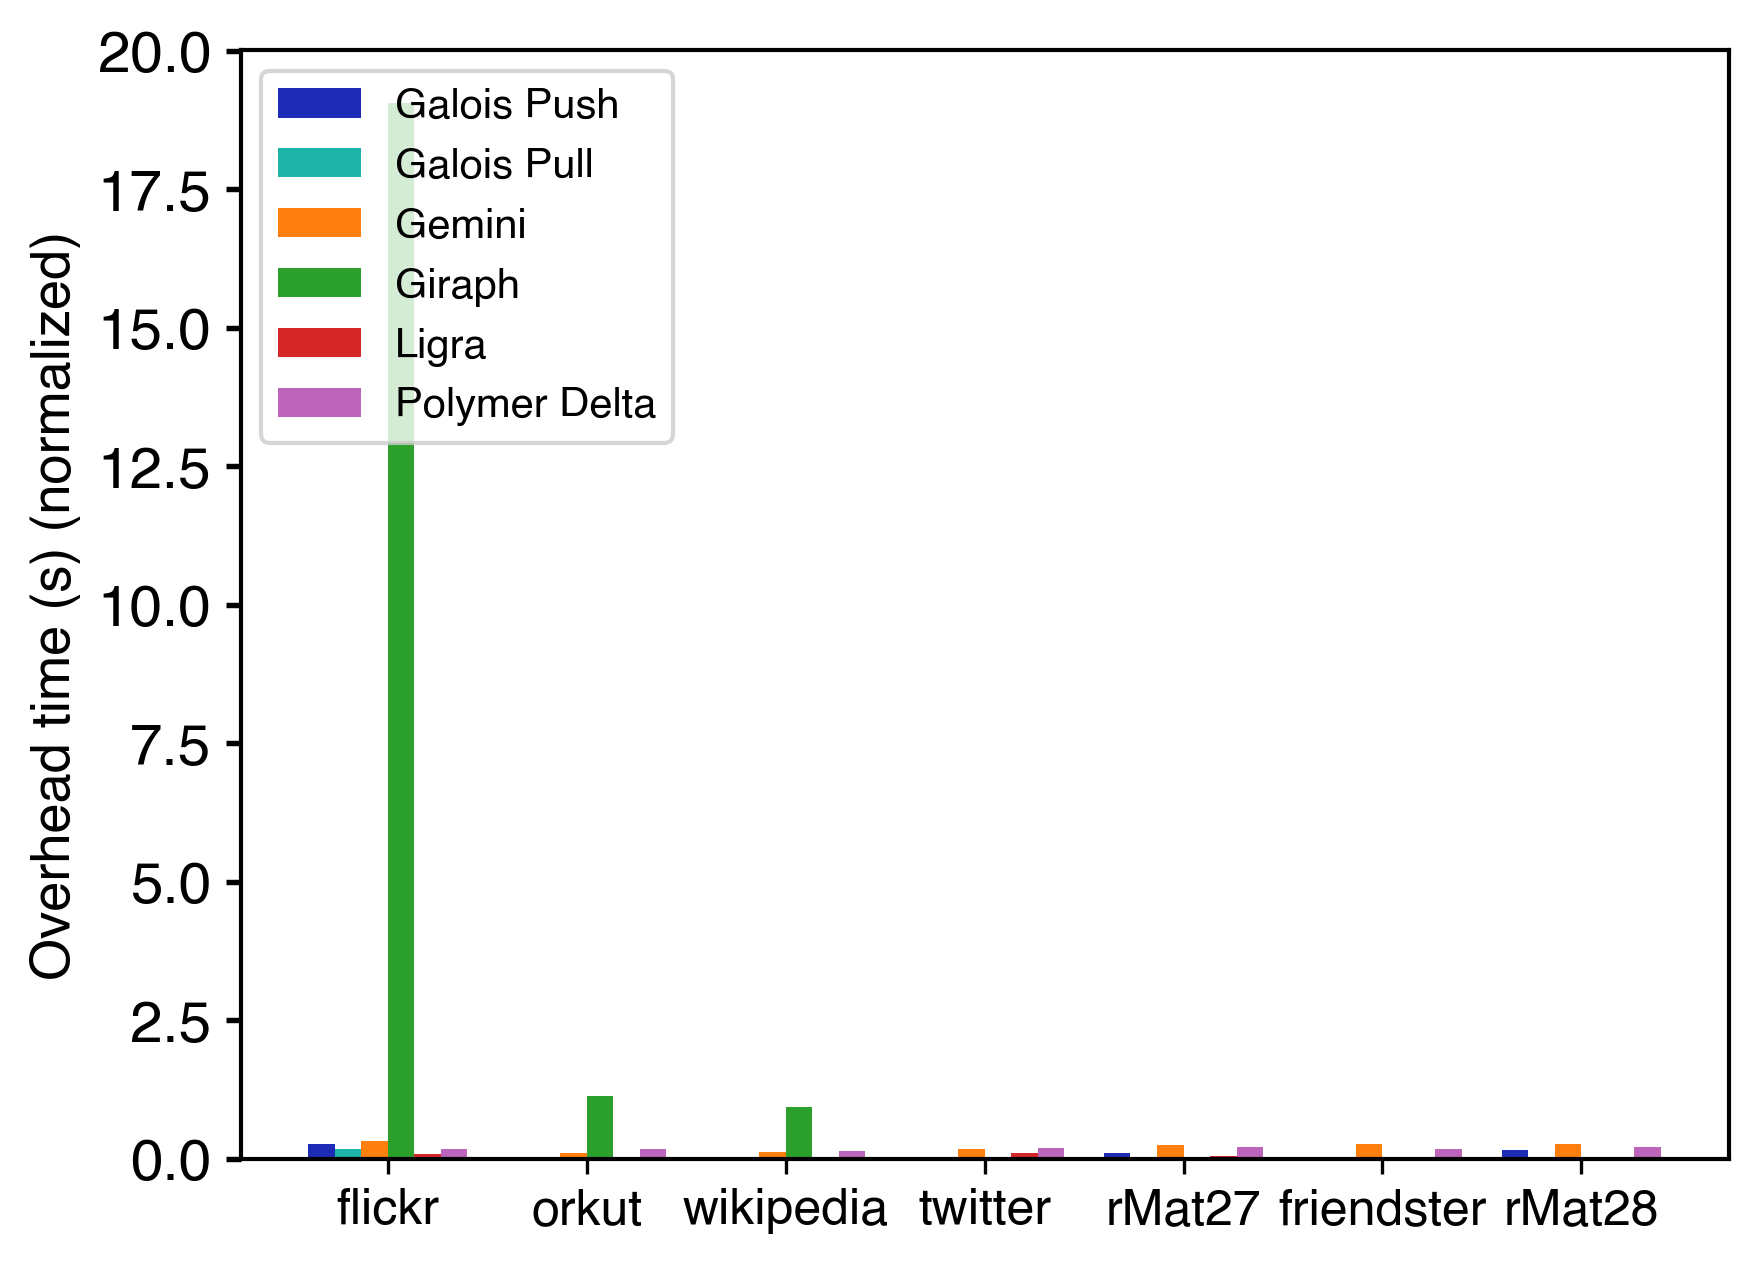
\includegraphics[width=\linewidth]{../../plots/singleNodePR_overheadTimeNormalized.png}
		\caption{Overhead time normalized by the graph size in million edges}
		\label{fig:singleNodePR_overheadNormalized}
	\end{subfigure}
	
	\caption{Average times on a single computation node, black bars represent one standard deviation in our testing}
\end{figure*}




\begin{figure*}
	\begin{subfigure}{0.3\textwidth}
		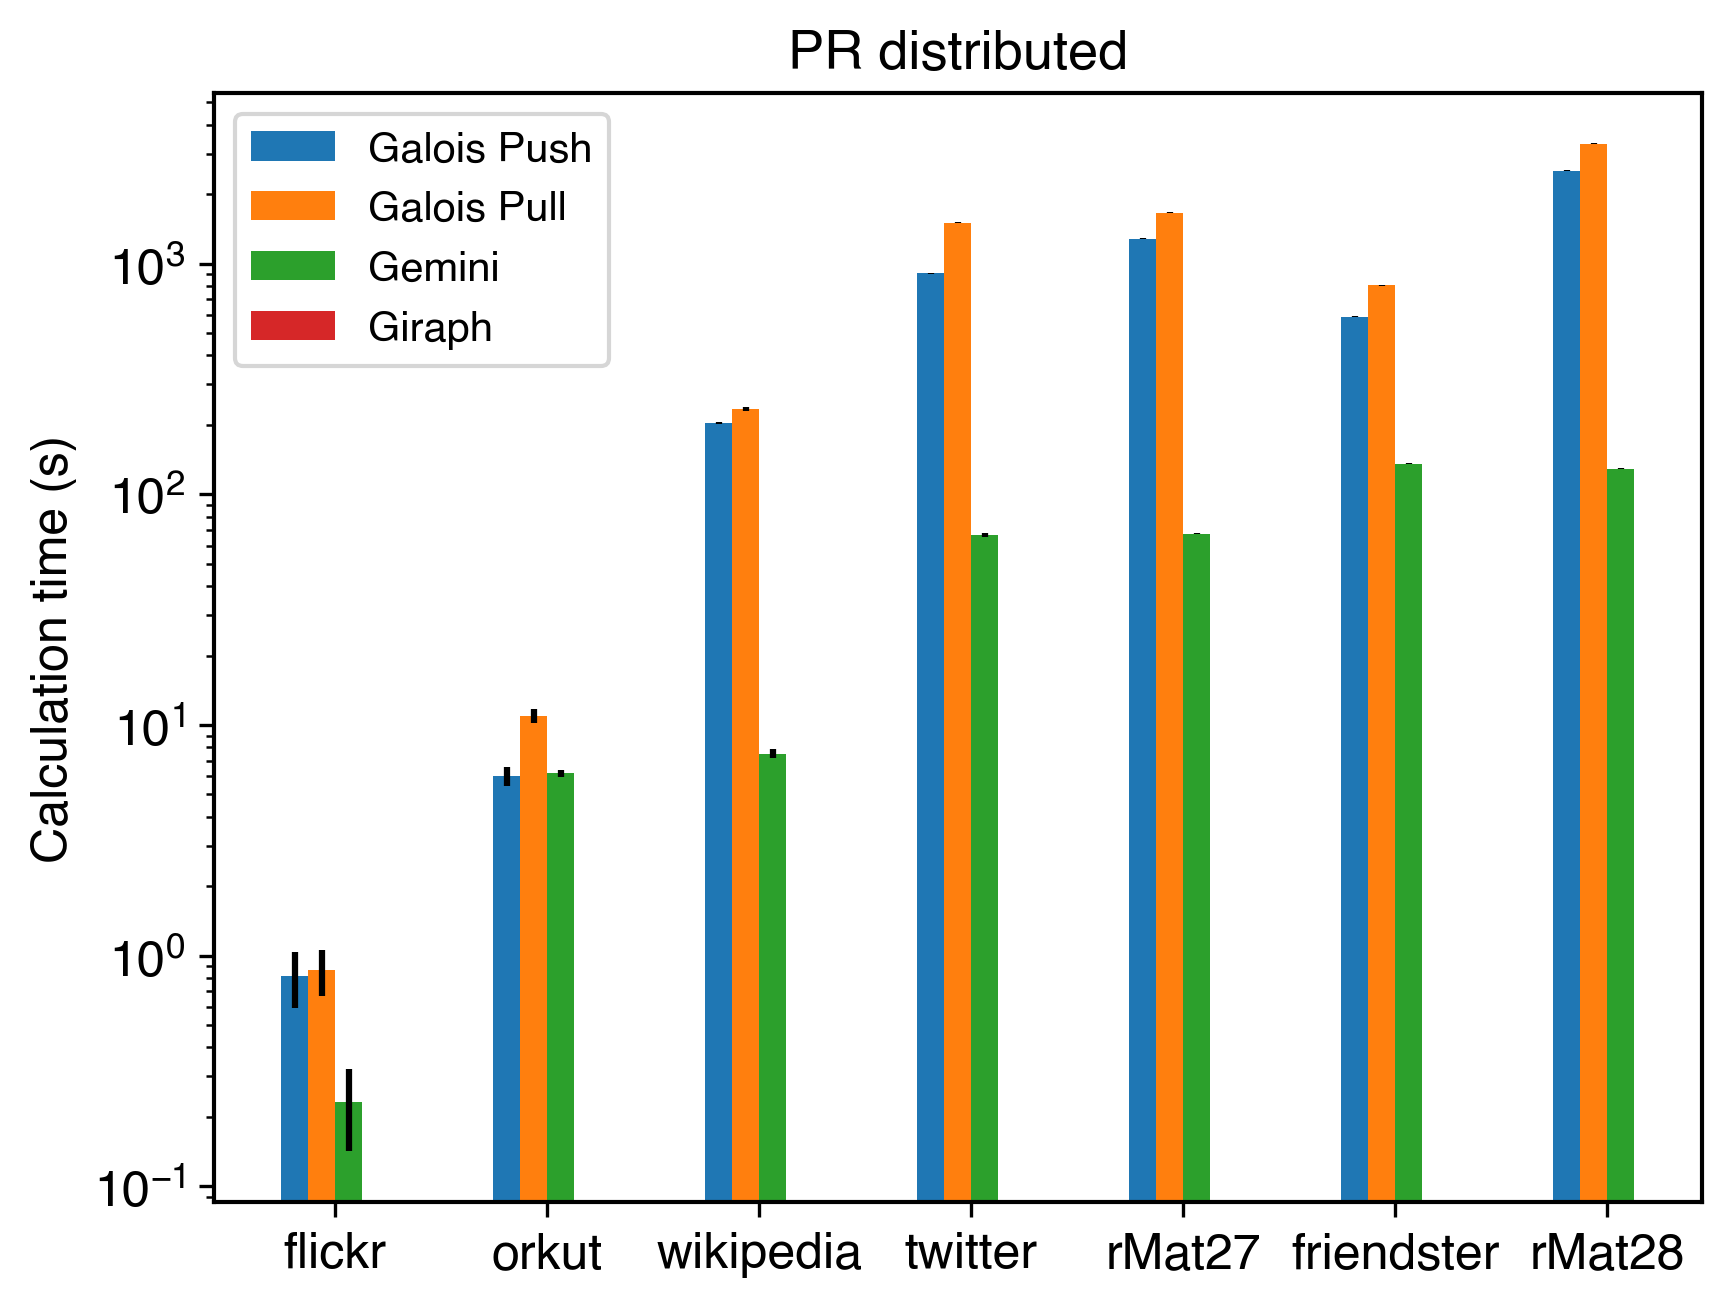
\includegraphics[width=\linewidth]{../../plots/distributedPR_calcTime.png}
		\caption{Calculation times for distributed PR}
		\label{fig:distributedPR_calc}
	\end{subfigure}
	\hfil
	\begin{subfigure}{0.3\textwidth}
		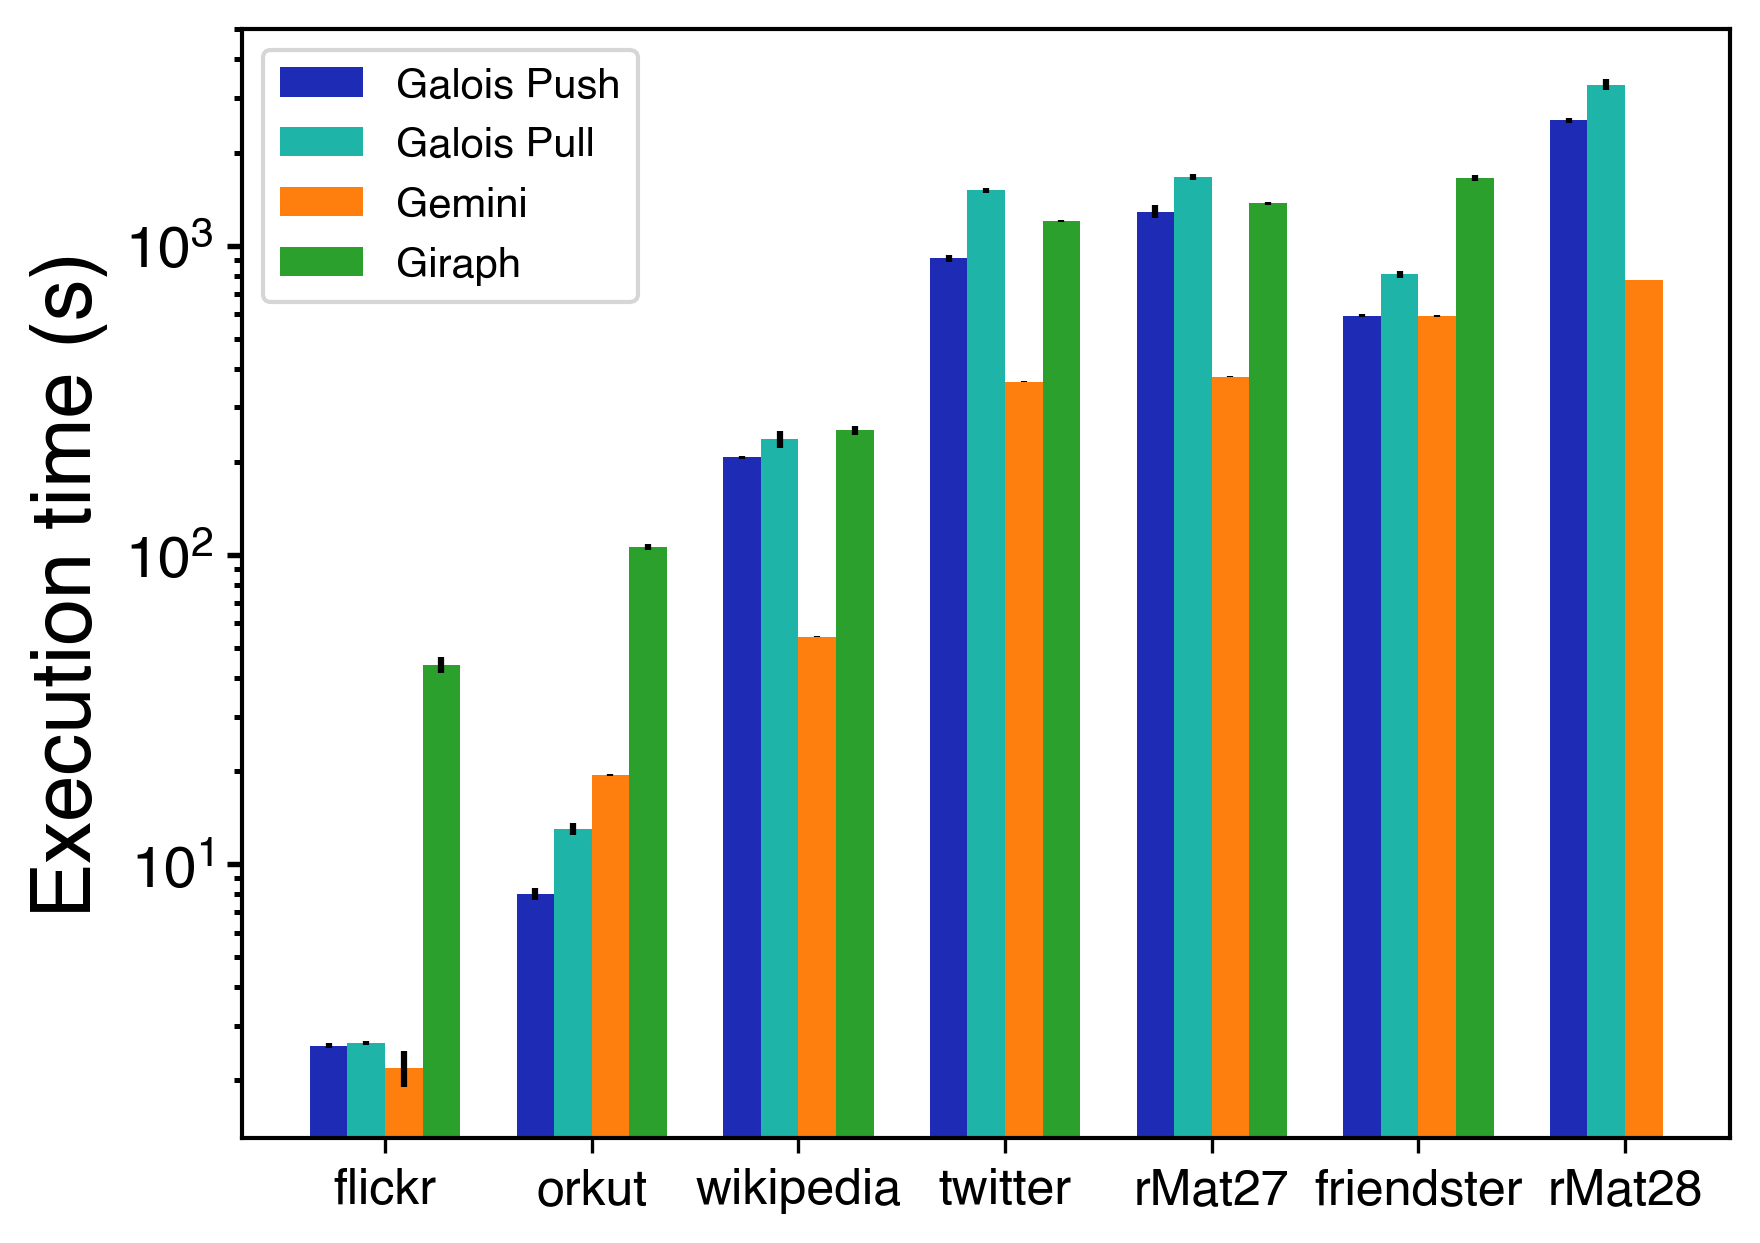
\includegraphics[width=\linewidth]{../../plots/distributedPR_execTime.png}
		\caption{Execution times for distributed PR}
		\label{fig:distributedPR_exec}
	\end{subfigure}
	\hfil
	\begin{subfigure}{0.3\textwidth}
		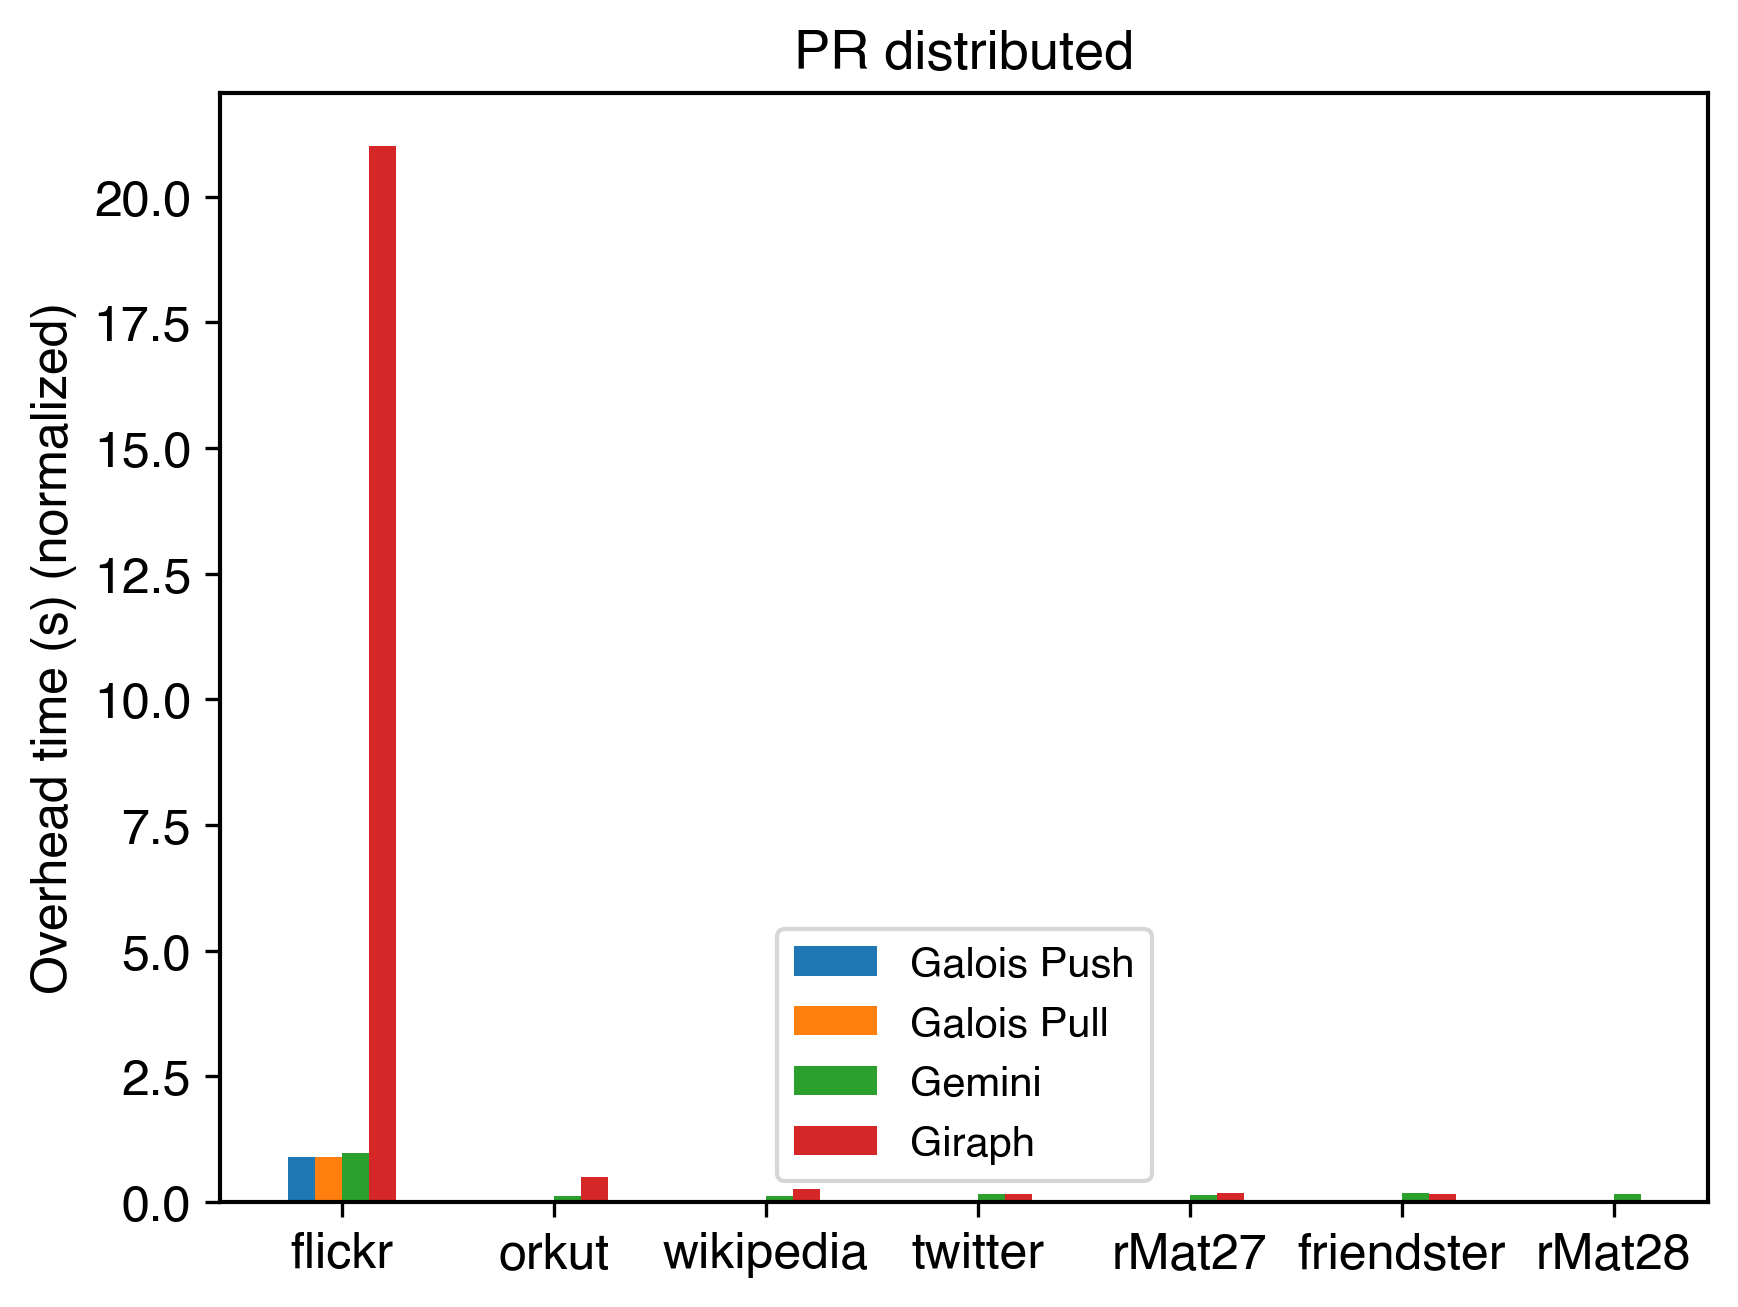
\includegraphics[width=\linewidth]{../../plots/distributedPR_overheadTimeNormalized.png}
		\caption{Overhead time normalized by the graph size in million edges}
		\label{fig:distributedPR_overheadNormalized}
	\end{subfigure}
	
	\caption{Average times on the distributed cluster, black bars represent one standard deviation in our testing}
\end{figure*}















\subsection{Galois speedup}
\label{sec:galois_speedup}
Analyzing the calculation time speedups for Galois, we can compare how or if the different algorithms benefit from increasing thread numbers.

\subsubsection{Single-source Shortest-path}
\begin{figure}
	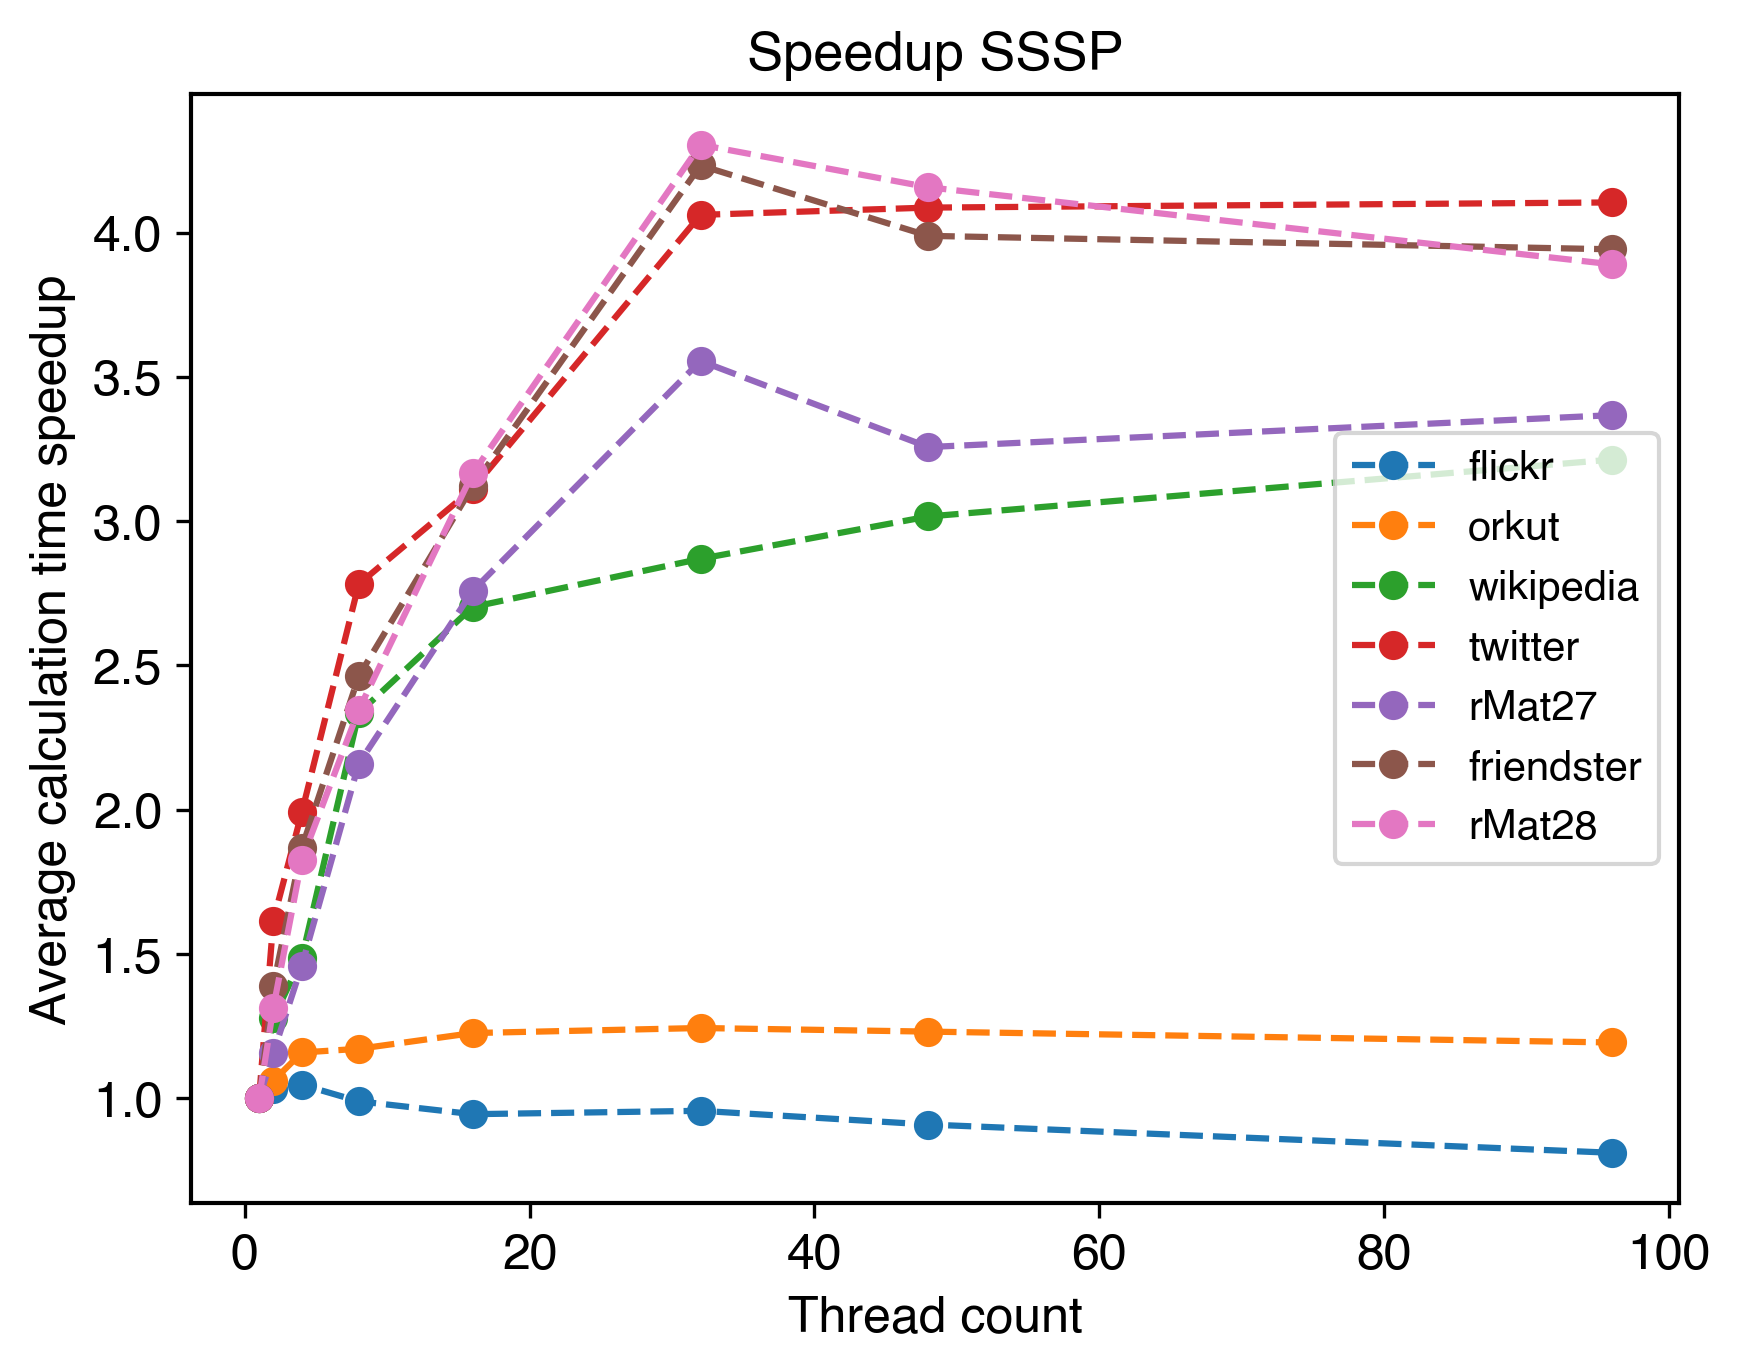
\includegraphics[width=\linewidth]{../../plots/singleNodeSSSPGaloisThreads.png}
	\caption{Calculation time speedup with increasing thread count for Galois Single-source Shortest-paths}
	\label{fig:galoisSpeedupSSSP}
\end{figure}
Starting with SSSP which is the algorithm that really is at an advantage when using many threads in \autoref{fig:galoisSpeedupSSSP}.

For all larger graphs, speedup is in most cases very close to optimal up to about 8 threads. 
Twitter has the best speedup, requiring only 38\%\ the calculation time with 2 threads compared to one, 25\%\ using 4 and 12.9\%\ using 8 threads.
Behaviour on friendster is similar with 52\%\ at 2 threads, 29\%\ at 4 and 16\%\ at 8 threads compared to one.

Anything above 32 threads however no longer helps decrease the computation time, in some cases even the opposite e.g. calculation on rMat28 is actually slower with 48 (13\% slower) or 96 threads (28\% slower) compared to 40 threads.

Small graphs like flickr or orkut, neither benefit from more threads nor is the performance held up by synchronization overhead. 



\subsubsection{Breadth-first search}
\begin{figure}
	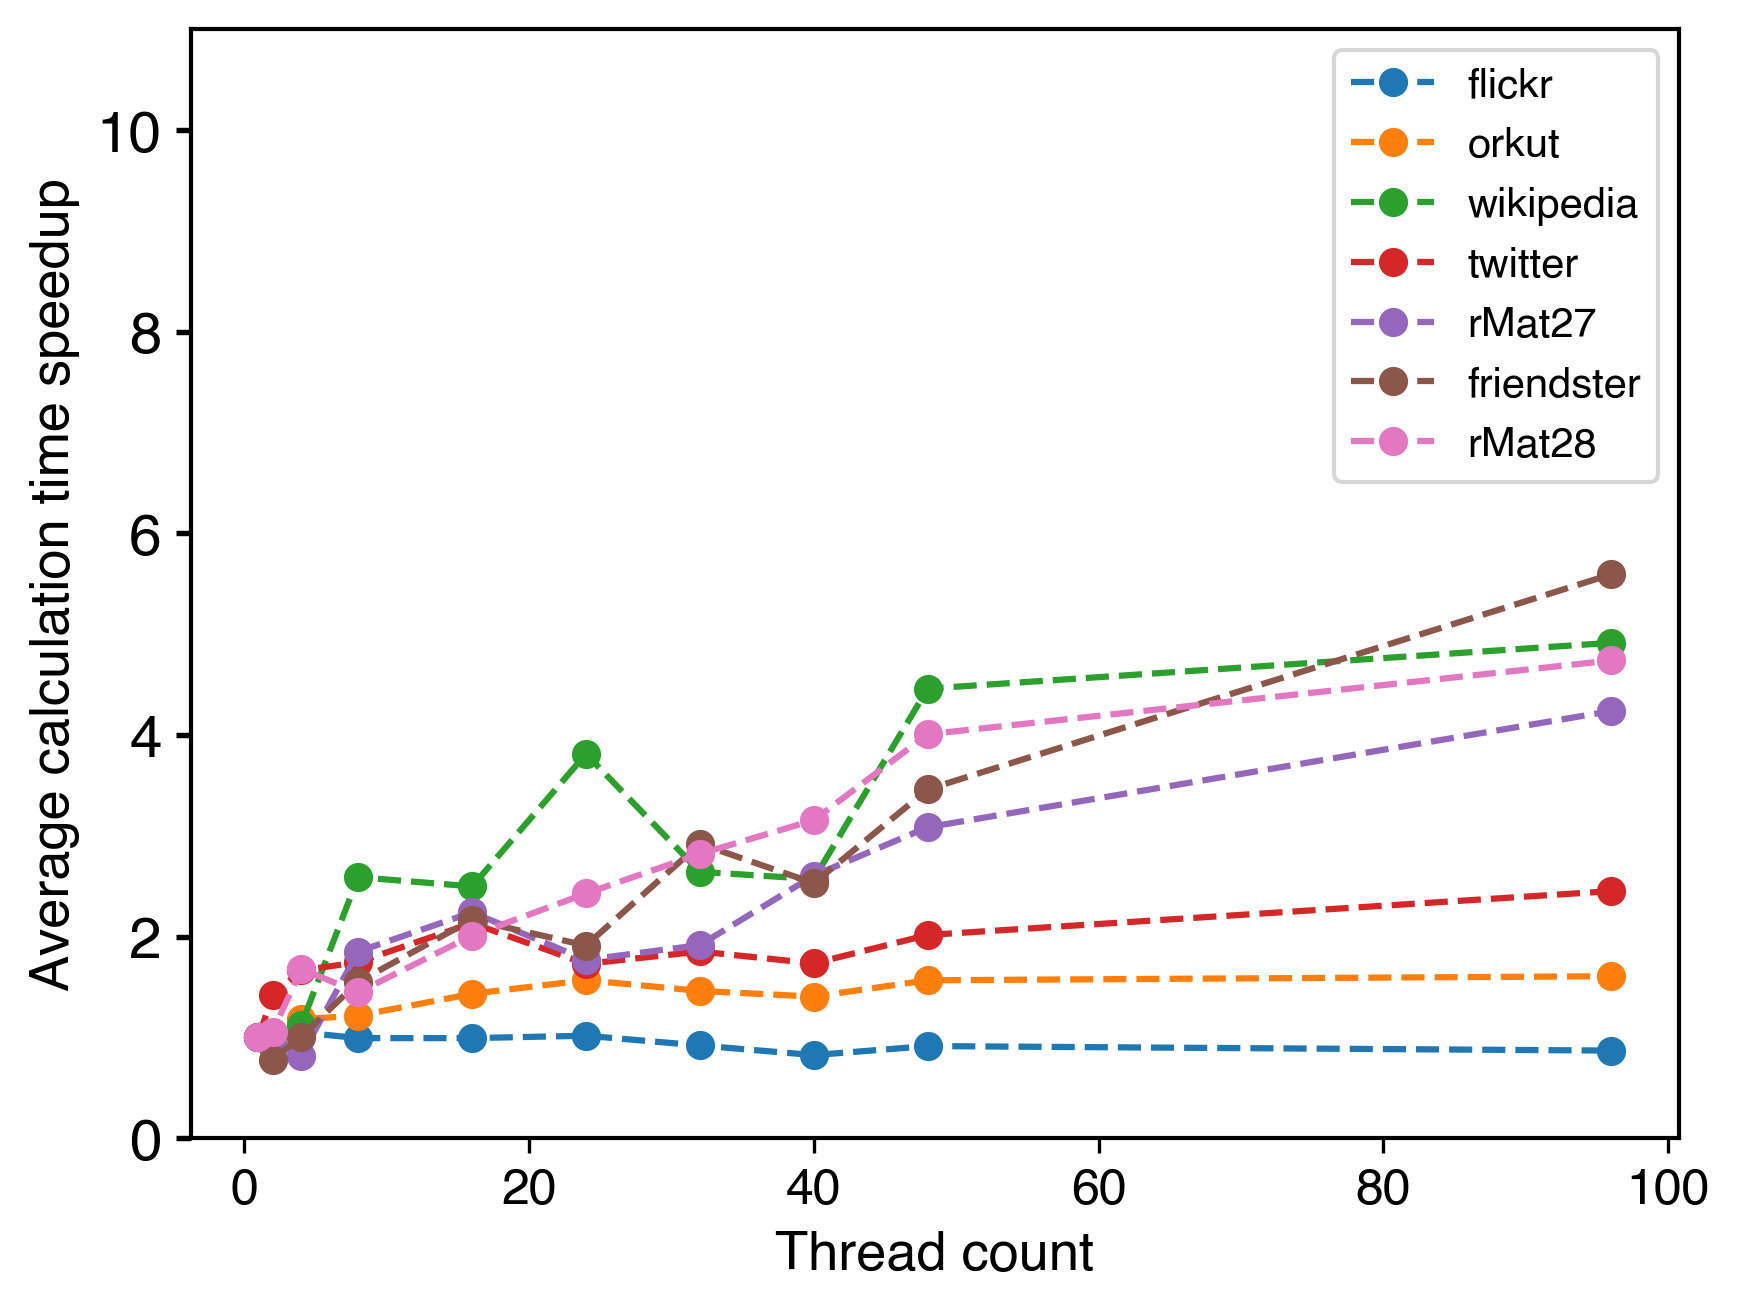
\includegraphics[width=\linewidth]{../../plots/singleNodeBFSGaloisThreads.png}
	\caption{Calculation time speedup with increasing thread count for Galois Breadth-first search}
	\label{fig:galoisSpeedupBFS}
\end{figure}








\begin{figure}
	\begin{subfigure}{\columnwidth}
		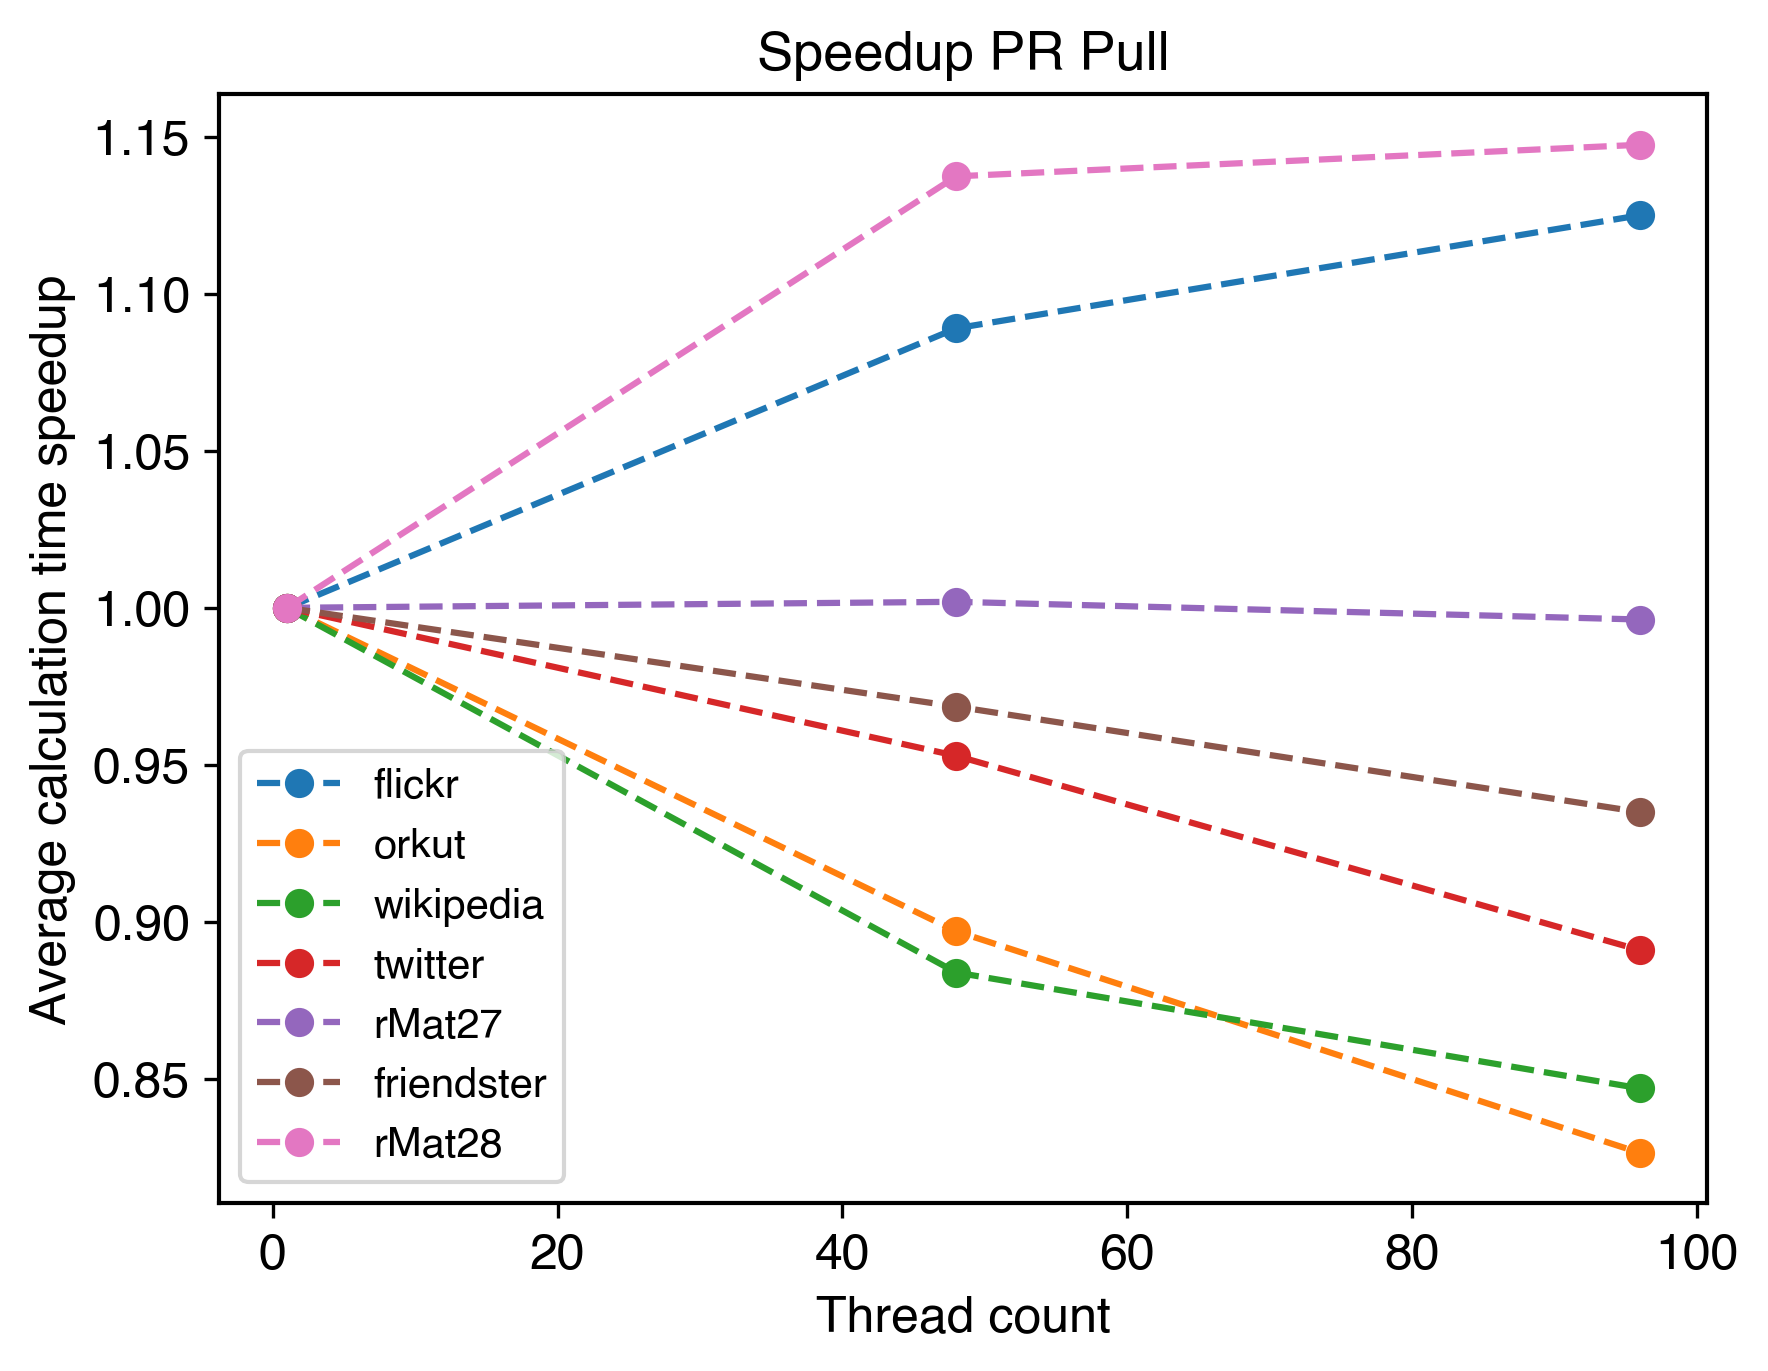
\includegraphics[width=\columnwidth]{../../plots/singleNodePRPullGaloisThreads.png}
		\caption{PageRank Pull}
		\label{fig:galoisSpeedupPRPull}
	\end{subfigure}
	\begin{subfigure}{\columnwidth}
		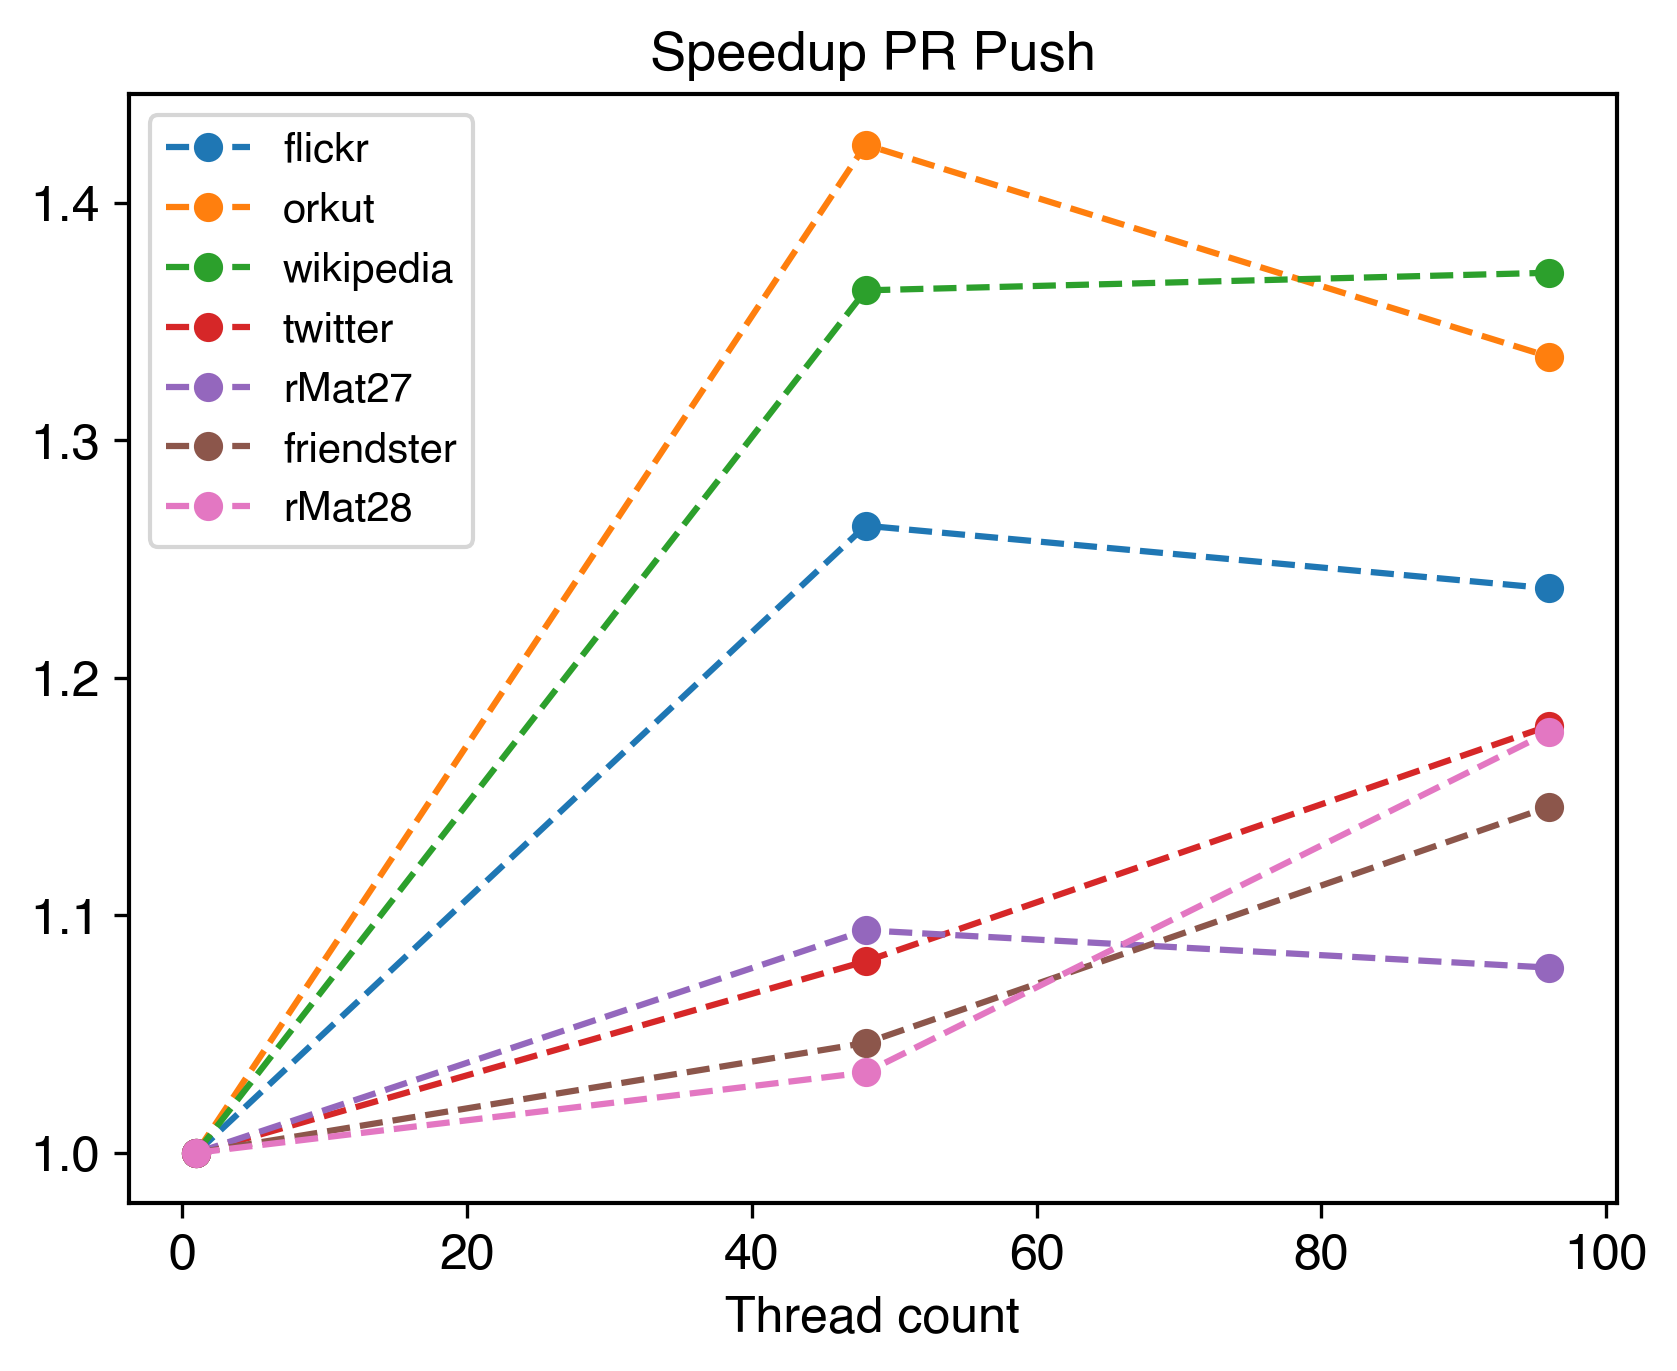
\includegraphics[width=\columnwidth]{../../plots/singleNodePRPushGaloisThreads.png}
		\caption{PageRank Push}
		\label{fig:galoisSpeedupPRPush}
	\end{subfigure}
	\caption{Calculation time speedup with increasing thread count for Galois PageRank Push and Pull algorithms.}
\end{figure}





\subsection{Execution times and overhead}



\begin{figure}
	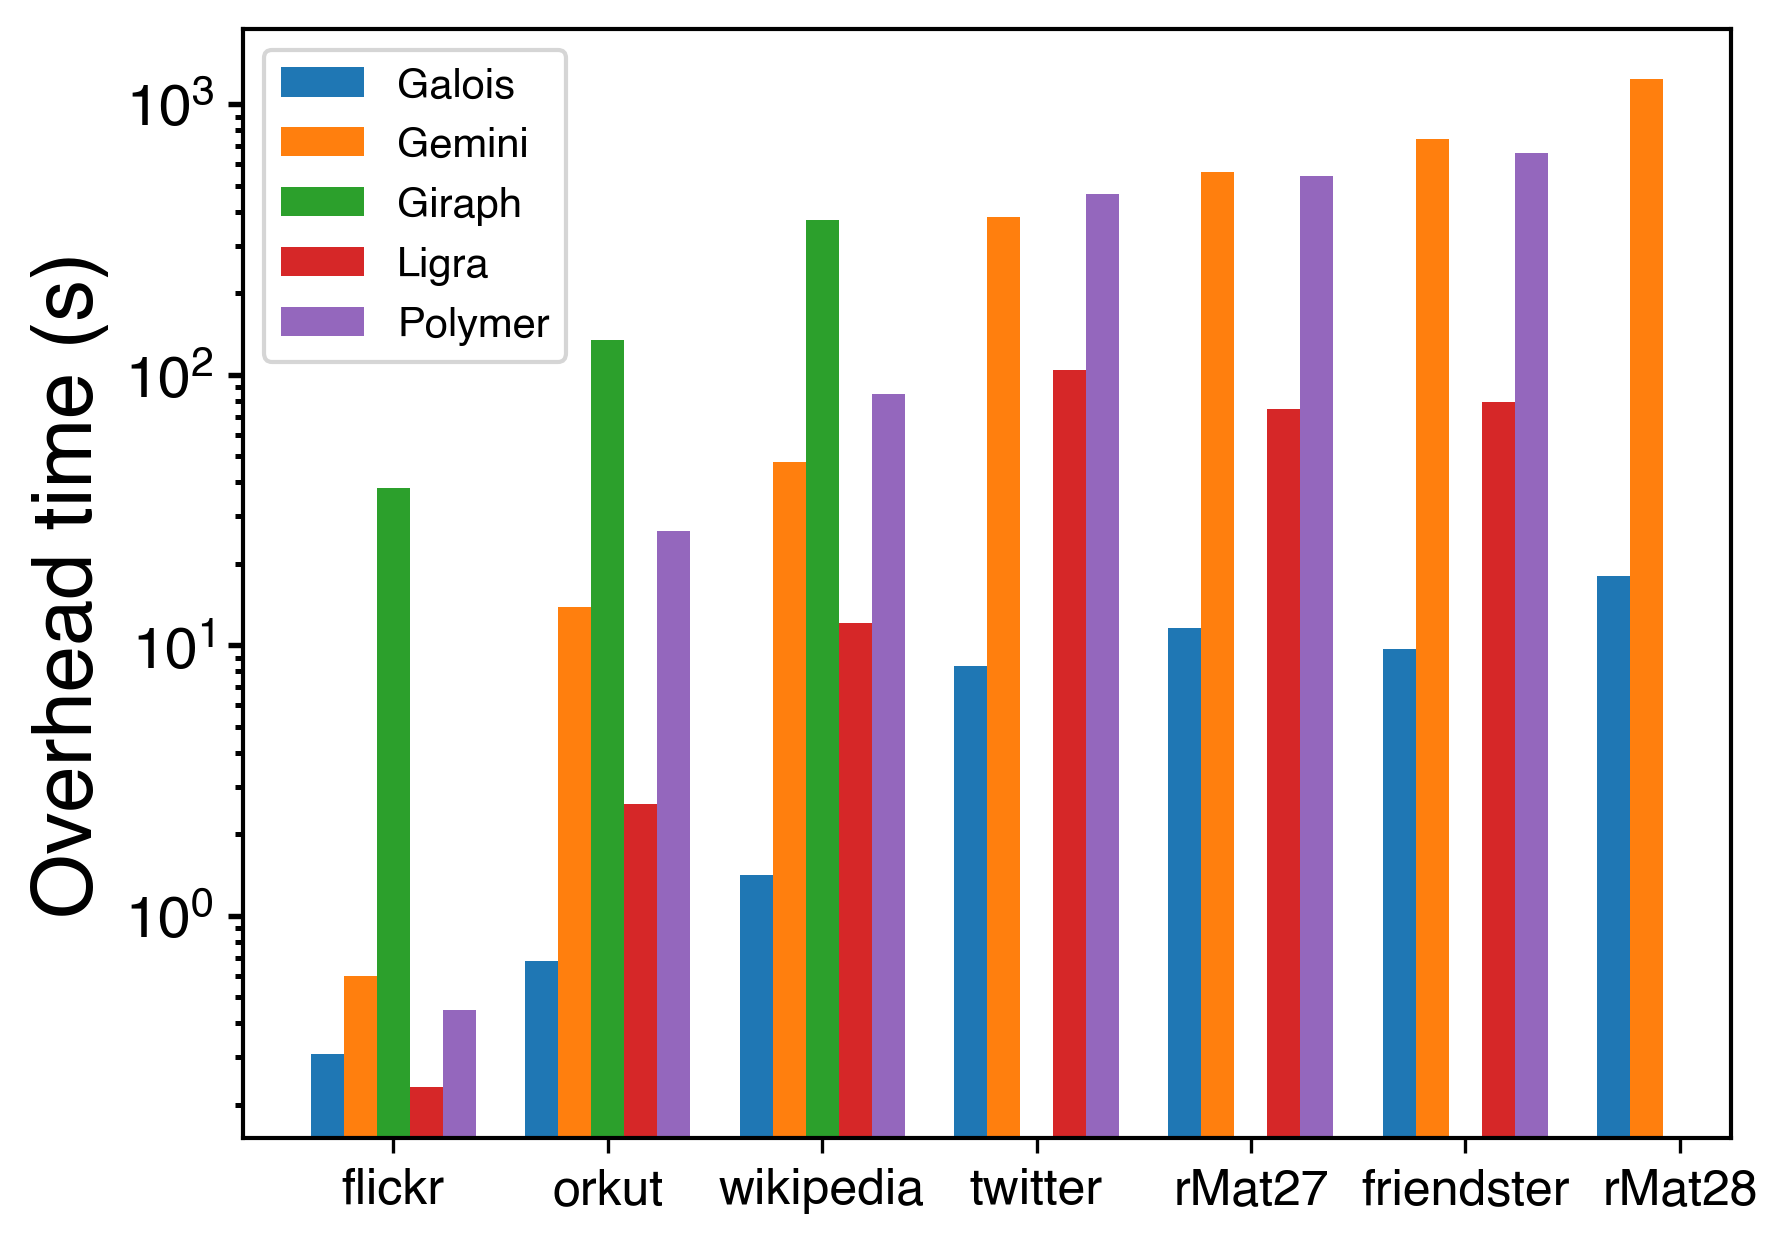
\includegraphics[width=\columnwidth]{../../plots/singleNodeSSSP_overheadTime.png}
	\caption{Overhead SSSP single node}
	\label{fig:singleNodeSSSP_overhead}
\end{figure}



\begin{figure}
	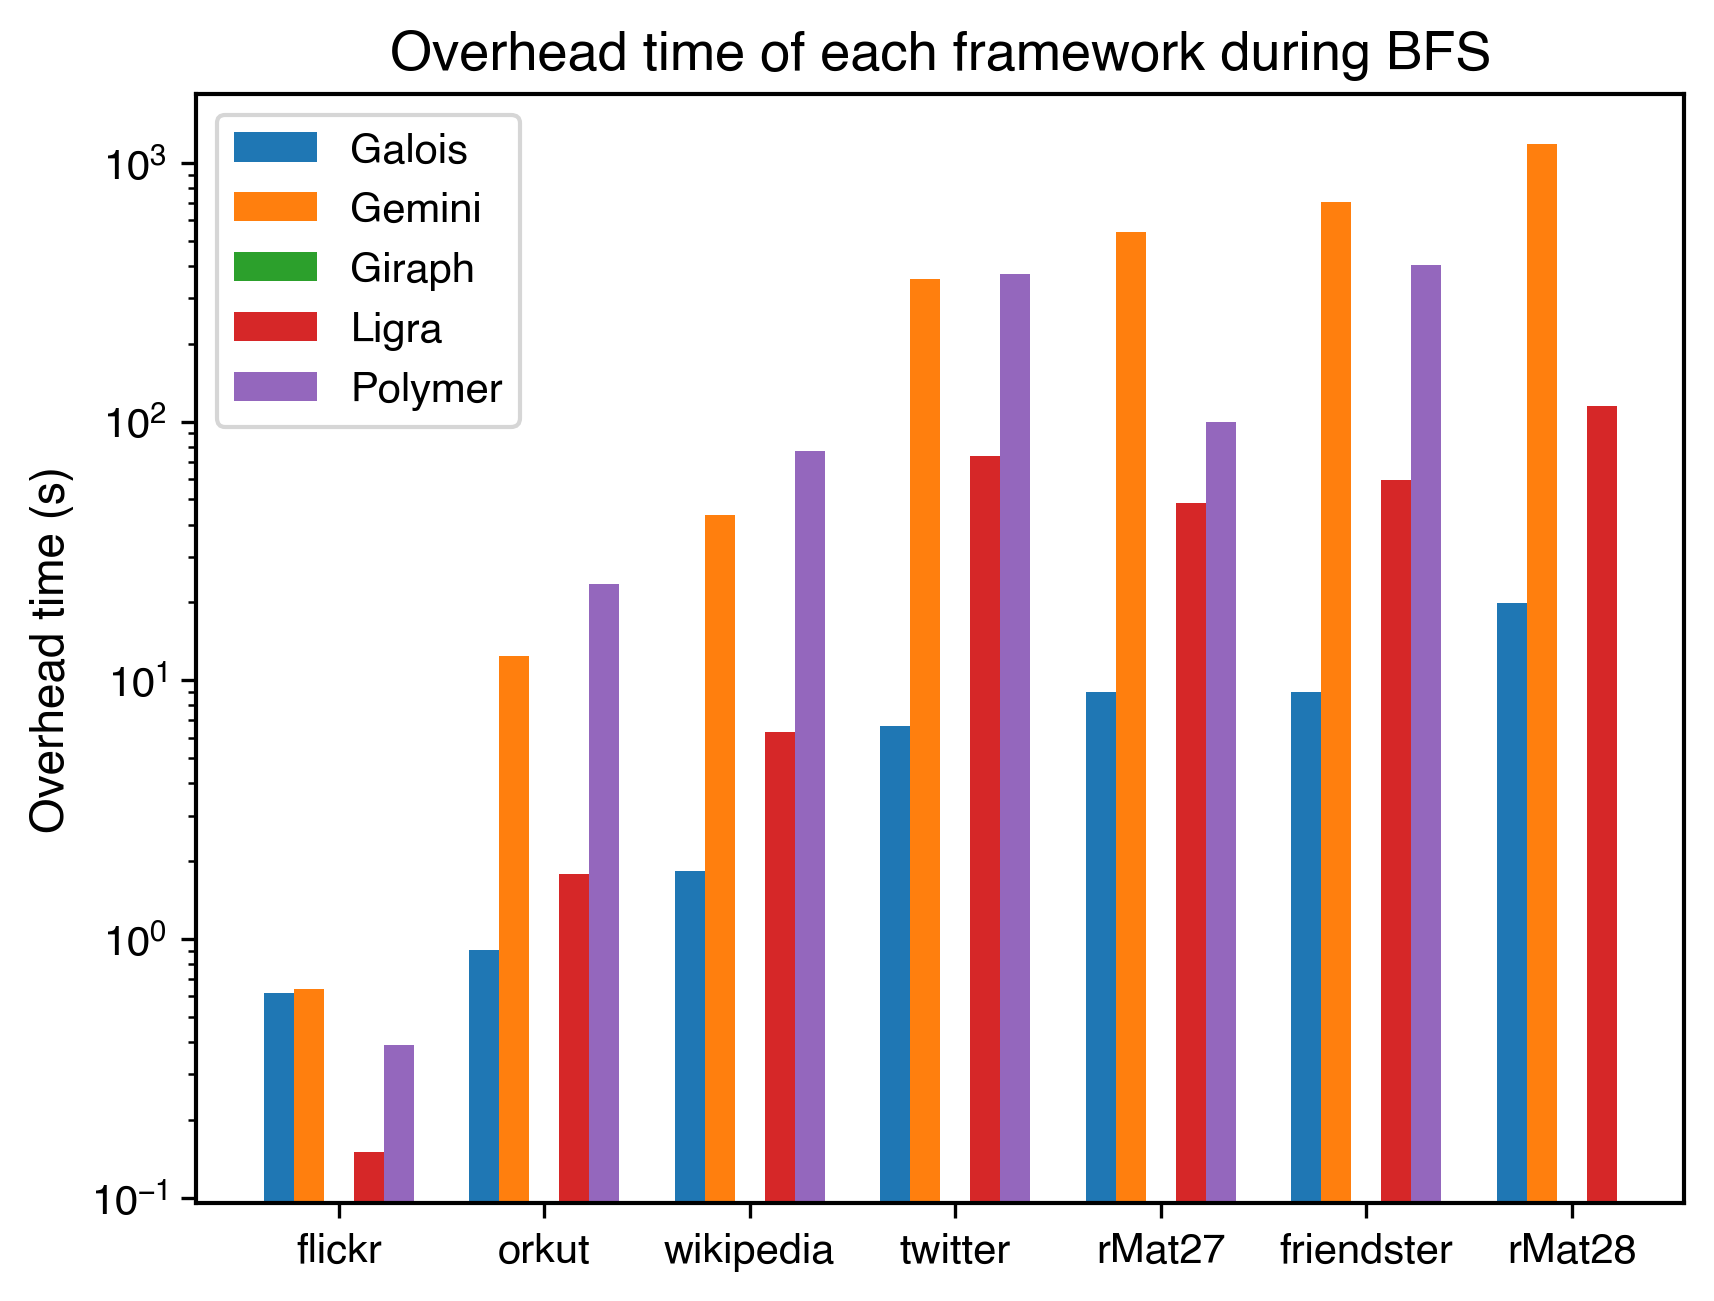
\includegraphics[width=\columnwidth]{../../plots/singleNodeBFS_overheadTime.png}
	\caption{Overhead BFS single node}
	\label{fig:singleNodeBFS_overhead}
\end{figure}



hier erhoffe ich mir einen Vergleich der Ladezeiten und erwarte, dass Systeme wie Giraph, die erstmal auf irgendwas warten schlecht abschneiden.
Aber vielleicht ist auch die setup time bei gleichen frameworks zwischen verteilt und shared memory ganz interessant zu vergleichen. 
